\documentclass[12pt,a4paper,oneside,openany]{book}

\usepackage{xcolor}
\usepackage{minted}
\usepackage[utf8]{inputenc}
\usepackage{tikz}
\usepackage{caption}
\usepackage{gensymb}
\usepackage{lmodern}
\usepackage{multirow}
\usepackage{booktabs}
\usepackage{array}
\usepackage{adjustbox}
\usepackage{upquote}
\usepackage{amsmath}
\usepackage{titlesec}
\usepackage[hidelinks]{hyperref}
\usepackage{fancyhdr}
\usetikzlibrary{mindmap,shadows, shapes, arrows, positioning}

%% Change these:
\newcommand{\projecttitle}{College Planner Web Application -- Built using the Java EE Platform}
\newcommand{\projectauthor}{Christopher Weir \\[0.2cm] Patrick Griffin \\[0.2cm] Gareth Lynskey \\[0.2cm] Paul Dolan}
\newcommand{\projectadvisor}{Kevin O'Brien, Gerard Harrison}
\newcommand{\projectprogramme}{B.Sc.(Hons) in Software Development}
\newcommand{\projectdate}{April 17, 2017}
%% End of things to change.



\tikzstyle{rect} = [rectangle, fill=blue!50, text width=4.5em, text centered, minimum height=4em, rounded corners]
\tikzstyle{line} = [draw, ->, very thick]
\tikzstyle{oval} = [ellipse, fill=green!50, text width=5em, text centered]

\newcolumntype{x}[1]{>{\centering\arraybackslash\hspace{0pt}}p{#1}}


\begin{document}
  \begin{titlepage}
    \begin{minipage}[t][6cm]{\textwidth}
      \centering
      \rule{\linewidth}{0.5mm} \\[0.4cm]
      { \LARGE \bfseries \projecttitle \\[0.4cm] }
      \rule{\linewidth}{0.5mm} \\[0.8cm]
    \end{minipage}
    
    \begin{minipage}[t][6.5cm]{\textwidth}
      \centering
      \textbf{\projectauthor}\\[0.5cm]
      \projectprogramme
    \end{minipage}
  
    \begin{minipage}[t][1cm]{\textwidth}
      \centering
      \textsc{\projectdate}
    \end{minipage}
      
    \begin{minipage}[t][3cm]{\textwidth}
      \centering
      \textbf{Final Year Project}\\[0.3cm]
      Advised by: \projectadvisor \\[0.1cm]
      Department of Computer Science and Applied Physics\\
      Galway-Mayo Institute of Technology (GMIT)
    \end{minipage}
  
    \begin{center}    
      
\includegraphics{img/gmit-logo.jpg}
    \end{center}
  \end{titlepage}
  \setcounter{page}{2}
  \tableofcontents
  %!TEX root = project.tex

\chapter*{About this project}
\paragraph{Abstract}
The aim of this project is to create a service that helps students with their college organisation as we believe, from personal experience over the last few years, that good organisation is key to a more improved academic performance. The approach taken to develop this service was to make a web application using the JEE (Java Enterprise Edition) with PostgreSQL and MLabs MongoDB. The services we chose to provide were a Calendar, Timetable, To-Do List, Module Tracker and Assignment Tracker. Users will be able to login or register to the web application, if a user is not logged in then they cannot access the web application. The Calendar will allow users to create, edit and delete events. The Timetable is fully customisable allowing for users to create their modules and add them to the timetable. The To-do lists purpose is to allow users to create tasks and check them off as they are completed. The Modules Tracker allows user to create modules and manage their grades for each module. The Assignment Tracker allows users to manage their assignments for each module they have created. These assignments also appear on the calendar. The purpose of the PostgreSQL database is to store user accounts, which can be edited or deleted through the users Profile page. The MongoDB database is responsible for storing each users’ data, this includes their data from all the services and their profile picture. The finished web application was uploaded on Heroku to allow for public access.

\paragraph{Authors}
This project has been developed by fourth year students: Christopher Weir, Gareth Lynskey, Patrick Griffin and Paul Dolan. We developed this project for our Bachelors of Science Honours Degree in Software Development. We divided up the work into four sections. Christopher, our Project Leader, handled the Registration and Login services. Gareth did the Timetable, Patrick the Calendar, and Paul the ToDo List and the Assignments page. Gareth, Chris, and Patrick worked on the Modules page together. We all collaborated on the database implementation, with each of us working on our respective sections on the database.

\chapter*{Acknowledgements}
We would like to acknowledge our team supervisors Kevin O'Brien and Gerard Harrison for support and understanding as well as all GMIT teachers for helping us to get this far.

\chapter{Introduction}
\par Throughout our three years of studying at Galway-Mayo Institute of Technology, we were embraced with the pressure of multiple Projects, Assessments, with struggled deadlines and trying to keep track of a list of different day to day tasks to be completed, whether college orientated or not. We have concluded that students need a more mobile and more accessible online platform for their academic organisation. Rather than having sheets of paper with lists or timetables we have created a system that incorporates numerous services for all students ranging from leaving cert level to third level students.

\par In order to get a sense of what we should incorporate into our system, we looked at what websites and mobile applications are currently available that offer college organisational support for students to use. Based on our findings we created a plan for our system. We used what we found to be the most suitable features from these websites and mobiles applications, along with introducing our own features that we believe would enhance the user experience of our system.

\par We wanted to create a way for students to track events, manage their college timetable, and keep track of assignments. We also understood that it is important for students to keep track of their college performance along with their overall Grade Point Average (GPA). Our plan was to have six key features which were a Calendar, Timetable, To-do List, Assignments Tracker, and a Modules Tracker to track your current progress within each Module.

\par Upon planning what we each wished to achieve from the creation of this system, we settle on gaining greater knowledge of the Java programming language. After further deliberation from our meetings we then decided that this system should be created as a web application developed in JEE which is Java Enterprise Edition. JEE provides the types of services that are necessary to build large scale, distributed, component based, multi-tier applications. Learning JEE was new to us in the sense of using JSP, Servlets and incorporating other technologies to build this web application\cite{SimonBrown}.

\chapter{Context}
The general context of this project is a system that provides several different but relative services to students to help them through their time at college. Students will be able to create an account through a simple registration process and they will even be able to customise their own profile. Student can create event on the calendar to help plan projects, etc. These events can be customised by colour coding for example and events can be displayed on three different views: Monthly, Weekly, and Daily. Students can create their own unique timetable for as we know personally, new timetables can be difficult to remember and adjust to. When a student has activities they must do, whether that be homework or extracurricular activities, they can keep track of these on their todo list and simply mark them off as they are completed. Students will be able to track their current academic progress by creating their modules and adding their results from projects or assessments to their respective modules. By doing this the students current progress for each module is calculated, along with their total Grade Point Average (GPA). Student can also monitor their assignments for each module that they have created. The students’ data is securely store on MLabs MongoDB and PostgreSQL databases which are hosted on Heroku. The application is secured using authentication codes allowing for no outside access to the application unless you are logged in.

\section{Objectives}
The overall objective of our project is to provide a college planner service that is both user friendly and intuitive in its design and functionality. Our web application was planned to contain multiple pages, and as such we deemed each page to be an objective as each page is a different service.

\begin{enumerate}
    \item \textbf{Login/Register Page:} The objective for the Login/Register page was to create a secure page to allow users to either login or register on the web application. This was to allow for database entries to be linked with a specific users account. The users account information is stored on a postgreSQL database and the users' data is stored on a MLabs MongoDB database, both of which are hosted on Heroku. This objective created more sub objectives which are as follows:
    \begin{itemize}
        \item Database Creation (postgreSQL, MLabs MongoDB)
        \item Authentication Filter
        \item Data Encryption
    \end{itemize}
    \item \textbf{AccountRecovery Page:} The AccountRecovery pages objective is to handle events where users may forget their account information, by allowing a means for resetting their account.
    \item \textbf{Profile Page:} The primary objective of the Profile page is to allow for a user to customise their profile, allowing for a greater user experience. The user can change their information and their profile picture, and can also delete their account if they so choose.
    \item \textbf{Calendar Page:} We wanted the Calendar to be simple to use, meaning a user could create, edit, and delete events just in a few clicks of a mouse. These events would be stored on the MongoDB database. The Calendar was to also have some customisable option such as colour coding events, along with being able to display assignments on their specific due dates.
    \item \textbf{Timetable Page:} The objective of the Timetable is to allow the user to create their own unique college timetable by adding Modules to it, which they could edit and delete with ease. The timetable entries are all stored on MongoDB.
    \item \textbf{Todo List Page:} We wanted the Todo List to be straightforward, the user can add entries, mark them as complete and remove them entirely. These entries are again stored on MongoDB.
    \item \textbf{Modules Page:} The objective of the Modules page is to allow the user to create Modules based on the module title and the module lecturer. The user can add results from assignments, exams, or projects to these Modules to calculate the result percentage. By adding these results the users’ total percentage for each module would be automatically calculated along with their total GPA based on these results. MongoDB would be responsible for storing this information.
    \item \textbf{Assignments Page:} The objective for the Assignments page is to keep track of the users' assignments based on the modules they created. Users' would be able to add and delete assignments.
\end{enumerate}

\section{Project Links}
Links to this write up report, the main project repository and the URL to the Web Application which is currently being hosted on Heroku, can all be found below.

\paragraph{Links}
\begin{itemize}
\item https://github.com/Chrissweir/Final-Year-Project/blob/master/project.pdf
\item https://github.com/Chrissweir/Final-Year-Project
\item https://collegeplannerfyp.herokuapp.com/
\end{itemize}

\section{Chapters Review}
In this chapter we will briefly review the different areas of this paper. From the design and planning phase to the implementation phase.

\subsection{Methodology}
In this chapter we will cover the different development methodologies we used to develop this project, including weekly project meetings, collaboration tools used, application testing and weekly meetings with the project supervisors.

\subsection{Technology Review}
The different technologies used to design and implement the project from start to finish. The software development approaches to the tools used to create our application and the particular reasons for choosing the specified technologies.

\subsection{System Design}
This chapter will provide detailed information about the application system itself along with how it functions. This chapter also covers the architecture of the project, data models used, along with diagrams and screenshots.

\subsection{System Evaluation}
This chapter describes how we believe that our application is secure and robust through testing techniques that were used to test the application. We also discuss our initial objectives compared to our achieved goals, and highlight any of the limitation or opportunities in the technologies used.

\subsection{Conclusion}
This chapter summarises the context of our project and the conclusion from the overall design and development of the project, we will review the final version of the application and discuss different parts of the implementation that could have been developed differently.

\chapter{Methodology}
This section describes the various stages of development that was undertaken throughout the duration of our College Planner web application. We will explain the thought process and methodologies carried out in order to come to an agreement on what project we would like to tackle. We will also go into detail regarding the languages, platforms and technologies used within this project along with the methods used to create this web application.

\section{Agile Development}
During the development of our project we took the agile approach as opposed to the more traditional approaches like the waterfall model or other approaches due to its flexibility. Change can be accepted through incremental, iterative phases called sprints. Therefore, requirements emerge and evolve as the application is developed. Each sprint delivers us user-desired, working, and new tested features. Each iteration generally consists of four distinct phases that include: planning, development, review, and retrospective.\par
It is well known that both estimating and planning are critical to the success of any software development project of any size or consequence. However, estimating and planning are not just about determining an appropriate deadline or schedule. Planning attempts to find a solution to the overall product development question: What should we build? In order for us to answer this question we had to take into account features, resources and our schedule. We could not answer this question all at once, it would have to be answered iteratively and incrementally. A good planning process reduces risk, reduces uncertainty, supports better decision making and establishes trust\cite{MikeCohn}.\par
In the planning phase, we held group meetings and decided and documented which new features are to be added to the software, or what changes we needed to make to existing software. We would keep track of these changes or creations using GitHub issues and milestones. We would allocate a team member to each task and give an estimated finish time. \par
In the development phase, everyone would work on the designing, testing, coding that was discussed in the planning phase. Then, in the user review phase, we would demonstrate our newly implemented features or changes to each other. We would then discuss if the software is correct and complete and remove the completed features from our GitHub issues and milestones and we would have another planning phase. Incomplete features are again assigned to an individual for future iterations. Lastly, in the retrospective phase, we all meet to reflect on the iterations and discuss improvements\cite{ChrisGeorge}.


\section{Version Control}
Throughout the development of this project we used GitHub, a free online version control service to help manage and keep track of all the changes to the source code. We divided the project into 4 sections, so we could all work on our own part. This worked perfectly with GitHub as we could create a branch for each of our sections of the project, and individually commit to those branches without interfering with each other’s branches and causing merge conflicts. When everyone was finished with making changes to their individual branch, Chris, our project leader would merge all the branches into the master branch, which contained all up to date sections of the project. When the master branch was up to date with all our source code, we would synchronize that version of the project onto our own individual branches. \par
GitHub was very helpful for setting up milestones for the project, i.e. Create a Login page. In each of these milestones we created git issues, which were multiple objectives we had to accomplish in order to complete the milestone as a whole. It really helped with breaking down the work load into smaller and more manageable segments.\par
Github was extremely valuable throughout the duration of this project by being able to visualise the changes made to the source code using the version control tool, in the event that we made an error and were unable to
undo that error in Eclipse. There were some instances where this happened and we needed to revert back to a certain commit in order to restore our previous version of the project to proceed with work. There is a built in command in the Git shell that allows you to revert back to a any specific commit so long as you had the commit identification code and the name of the branch of which you wanted to revert back to, which was very helpful through the development of the project.

\section{Testing}

When deciding which frameworks we would like to use to validate and test our web application, our team reached an agreement that we would use both Selenium IDE and Junit to carry out this process. Selenium allows you to record, edit and debug tests. We had a previous understanding of Selenium as we had used it in third year which benefitted us. We tested every web page which included testing navigation, add, edit and delete. One all the tests had passed we then went about creating test suites which runs through all the test cases. Along with Selenium, we integrated Junit testing into our web application.
\par When we set out brainstorming this project, we appreciated the fact that there was a range of different algorithms, languages, technologies and frameworks that we could use to develop our web application. When deciding what primary language to programme College Planner in we came to a mutual agreement that we were all comfortable using java seeing as this was the dominant coding language we practiced over the last four years and we also wanted to improve our understanding of the language. The Java programming language is the most common known language worldwide\cite{MonicaPawlan}. We chose to use java for many reasons mainly because of its Object-Oriented programming which we would be demonstrating in our web application, portability as it runs on almost anything and java also has satisfying support for HTML, SQL and XML built in, all of which we used in our web application. Being able to see our errors due to error messages at compile time was also invaluable throughout the duration of our project as we could single out where we had made our mistake. \par 
Having previous knowledge of MongoDB stood to us during the development of our project and that along with it being document based which made it more suitable over using a file server helped us in making a decision when choosing a database to use for our project. MongoDB has a range of features that were beneficial to us throughout the duration of this project including file storage, ease of scale-out, replication and high availability, auto sharing and deep query availability in that MongoDB supports dynamic queries on documents using a document-based query language that's nearly as powerful as SQL\cite{Mongo}.


\chapter{Technology Review}
In this section, we're going to discuss the technology used throughout the development of this project. This section will briefly cover the technologies and the benefits of choosing these technologies. 


\section{Development Environment}
Throughout the duration of this project we used a range of different programming tools to create our College Planner web application. To complete this project, we combined a range of features in order to programme, host, test and manage College Planner all of which are explained below. 

\subsection{Eclipse EE}
Eclipse is an integrated development environment (IDE) with an extensive number of plug-ins used for customizing the programmer’s environment. It contains a base workspace for the programmer to keep track of their work and existing projects. Eclipse is predominantly Java based i.e. it's written in Java and mostly used for developing Java applications. The Eclipse IDE for Java EE is used for developing Java EE applications, it has editors from HTML/JSP and JavaScript. Java EE features things such as integration with Tomcat or other Servlet engines\cite{Eclipse}. 

\subsection{Heroku CLI}
Formerly known as the Heroku Toolbelt, the Heroku Command Line Interface is a tool that wraps the Heroku Platform API, providing support for various things like creating and managing Heroku applications, running one-off dynos, taking backups, and configuring add-ons all from the command line / shell of different operating systems. The Heroku CLI automatically keeps itself up to date. When a Heroku command is run in the terminal, a background process will be initialised that checks the URL for the latest version of the CLI\cite{HerokuCLI}. If a newer version exists, it will be downloaded and stored in the ~/.local/share/heroku/cli directory. The background check will initiate at most every 4 hours. Before loading system-installed version, the heroku binary will check for updated clients in ~/.local/share/heroku/cli.\\
\\
The following are some sample Heroku CLI commands:

\begin{itemize}
    \item heroku login\par
    Login to your Heroku account.
    \item heroku create example\par
    Creating an app named example.
    \item heroku plugins:install heroku-cli-deploy\par 
    Install the heroku cli deploy plugin.
    \item heroku war:deploy <path\_to\_war\_file> --app <app\_name>\par
    Deploy a .war file to a specific app on heroku.
\end{itemize}

\subsection{GitHub}
GitHub is a web-based Git or version control repository and Internet hosting service that was founded in 2008. GitHub offers distributed version control,
source code management (SCM), access control and many other collaboration features such as bug tracking, feature requests, task management, documentation, commits history, and wikis for every project\cite{KlintFinley}. GitHub provides both public and private repositories which are used to
host open-source software projects. Public repositories are free to use but private repositories come at a fixed monthly cost. GitHub also provides a graphical user interface for Windows and Mac, GitHub Desktop App to help eliminate the use of the command line tools for managing project uploads and commits, but many others prefer using the command line tool Git for this.\\
\\
Some sample git commands used are as follows:
\begin{itemize}
    \item git clone path/to/repo\par
    This command allows to clone any project from your github account
    or any publicly available project for that matter.

    \item git clone path/to/repo\par
    This command allows to clone any project from your github account
    or any publicly available project for that matter.
    
    \item git status\par
    Checks the status of project once it has been cloned it shows
    added deleted and modifies files as well as indicates which files
    are tracked.
    
    \item git add .\par
    Add folders or files to be tracked by github so later they can be
    committed and pushed on to github account.
    
    \item git commit –a\par
    Makes local commit of all the changes done in folder added by
    previous command git add .
    
    \item git push origin master\par
    Pushes commit (git commit -a) to users github account on his/her
    account
    
    \item git push origin +'COMMIT ID':master\par
    Reverts back to the state of the repo at the desired commit
\end{itemize}

\subsection{JUnit}
Junit is a framework that is used to write repeatable tests. Used for the Java programming language, JUnit an instance of the xUnit architecture for unit testing frameworks. JUnit has been imperative in the development of test driven development which is part of a larger software design archetype know as Extreme Programming(XP). Junit consists of a graphical user interface (GUI) which makes it possible to write and test source code easily. Junit allows the user to incrementally build test suites which measures the progress while detecting unintended side effects. Junit tests contains a progress bar that is green when passes and red when it fails. Multiple tests may be run concurrently and the simplicity of Junit allows the user to easily correct bugs as they are found\cite{JUnit1}.\\
\\
A sample JUnit test case can be found below\cite{JUnit}:

\begin{minted}{java}
import static org.junit.jupiter.api.Assertions.assertEquals;
import org.junit.jupiter.api.Test;

public class MyTests {

    @Test
    public void multiplicationOfZeroIntegersShouldReturnZero() {
        MyClass tester = new MyClass(); // MyClass is tested

        // assert statements
        assertEquals("10 x 0 must be 0", 0, tester.multiply(10, 0));
        assertEquals("0 x 10 must be 0", 0, tester.multiply(0, 10));
        assertEquals("0 x 0 must be 0", 0, tester.multiply(0, 0));
    }
}
\end{minted}

\subsection{Selenium}
Selenium-IDE (Integrated Development Environment) is a tool which is used to develop Selenium test cases. Selenium IDE consists of a Firefox plug-in and is commonly the most adequate measure of developing test cases. It contains a context menu which allows you to select a UI element from the browser’s currently displayed page and then selects from a pre-defined list of Selenium commands with parameters according to the context of the selected UI element. This does not only save time but is also an exceptional way of learning Selenium script syntax. Selenium IDE supports autocomplete mode when creating tests. This aspect benefits the tester as it helps to enter commands quicker and also restricts the user from entering invalid commands\cite{Selenium}.


\section{Java EE}
The official documentation defines Java Platform, Enterprise Edition or 
Java EE as a widely used computing platform for developing, building and 
deploying Web-based enterprise applications online, which was formerly known as Java 2 Platform, Enterprise Edition 
or J2EE \cite{JavaEE}.
\par
The Java EE platform is built on top of the Java SE platform, which provides an API for object-relational mapping and runtime environment for developing large-scale, reliable, multitiered, scalable and secure web applications\cite{JEEJSE}.
At a client tier, Java EE supports Java applets or applications, as well as HTML. It depends on Java Servlet Pages and servlet code to create and process HTML or other formatted data for the client\cite{VangieBeal}.
\subsection{JSP}
JavaServer Pages is a technology that provides web developers with a framework to create dynamically generated web pages using HTML, XML and java code which is secure, fast and independent of server platform \cite{ScottMcPherson}. JSP is similar to PHP and ASP but uses the java programming language.
\par
JavaServer Pages have dynamic scripting capabilities that work in conjunction with HTML code, which seperates the page logic from the static elements (the actual design and display of the page), to help make the HTML more functional\cite{JSP}. In order to deploy and run JavaServer Pages, a compatible web server with a servlet container, such as Apache Tomcat is required.\\
\\
\textbf{Example\cite{Pankaj}:}
\begin{minted}{jsp}
<%@ page language="java" contentType="text/html; charset=US-ASCII"
    pageEncoding="US-ASCII"%>
    <!DOCTYPE html PUBLIC "-//W3C//DTD HTML 4.01 Transitional//EN"
    "http://www.w3.org/TR/html4/loose.dtd">
    <html>
        <head>
            <meta http-equiv="Content-Type" 
            content="text/html; charset=US-ASCII">
            <title>First JSP</title>
        </head>
        <%@ page import="java.util.Date" %>
        <body>
            <h3>Hi Pankaj</h3><br>
            <strong>Current Time is</strong>: <%=new Date() %>
        </body>
    </html>
\end{minted}
\subsection{Servlets}
A servlet is a java program that extends the capabilities of a server. Although a servlet may respond to any type of request, they most often implement applications on web servers\cite{ErikJendrock}. Servlets are most commonly used to process and store a Java class in Java EE that conform to the Java Servlet API. The Java Servlet API, contained in the javax.servlet and javax.servlet.http package hierarchies,
define the expected interactions of the web content and servlet\cite{StefanZeiger}.
Web servlets are java version of other dynamic web content technologies such as PHP and ASP.NET. Below is a sample of a servlet \cite{ServletExamples}.

\begin{minted}{java}
// Import required java libraries
import java.io.*;
import javax.servlet.*;
import javax.servlet.http.*;

// Extend HttpServlet class
public class HelloWorld extends HttpServlet {
 
  private String message;

  public void init() throws ServletException
  {
      // Do required initialization
      message = "Hello World";
  }

  public void doGet(HttpServletRequest request,
                    HttpServletResponse response)
            throws ServletException, IOException
  {
      // Set response content type
      response.setContentType("text/html");

      // Actual logic goes here.
      PrintWriter out = response.getWriter();
      out.println("<h1>" + message + "</h1>");
  }
  
  public void destroy()
  {
      // do nothing.
  }
}
\end{minted}



\subsection{XML}
XML stands for Extensible Markup Language. XML was designed to store and transport data and to be both human- and machine-readable\cite{XMLtutorial}. XML data is known as self-describing or self-defining, meaning that the structure of the data is embedded with the data, thus when the data arrives there is no need to pre-build the structure to store the data; it is dynamically understood within the XML\cite{MargaretRouse}. The following is an example of XML\cite{NormanWalsh}:

\begin{minted}{xml}
<configuration-file>
    <section name="section1">
      <entry name="name1" value="value1"/>
      <entry name="name2" value="value2"/>
    </section>
    <section name="section2">
      <entry name="someothername" value="someothervalue"/>
    </section>
  </configuration-file>
\end{minted}

\subsection{Apache Tomcat}
Apache Tomcat, often referred to as Tomcat, is an open source Java Servlet Container that implements several Java EE specifications including Java Servlet, JavaServer Pages, Java Expression Language and Java WebSocket technologies\cite{ApacheTomcat}. Tomcats core component is the servlet container Catalina, when the Tomcat server is being started it is actually Catalina being started. Catalina implements Sun Microsystems' specifications for servlet and JavaServer Pages (JSP).

\section{Heroku}
Heroku is a container-based cloud Platform as a Service. Heroku is used by developers to deploy, manage and scale modern apps. Heroku’s platform is elegant, flexible and manageable which offers developers a straightforward path when getting their apps to market. This was an obvious benefit to us when choosing what platform to integrate into our project. Heroku is fully managed which gives developers the freedom to focus on their core product without having to maintain servers, hardware, or infrastructure. Heroku provides services, tools, workflows, and polyglot support all of which enhances the developer’s productivity\cite{Heroku}.
 

\subsection{MongoDB}
MongoDB is a free, open source cross-platform database program. It is document-oriented which means it is designed for storing, retrieving, and managing document-orientated information. This is also known as semi structured data. MongoDB is a NoSQL database program and uses JSON-like documents with schemas. MongoDB is a distributed database and is designed for ease of development and scaling it also possesses satisfying scalability and flexibility. The document model maps to the objects in your application code which makes data easy to work with. Ad hoc queries, indexing, and real time aggregation provide powerful ways to access and analyse your data \cite{MongoAbout}. \par MongoDB provides a wide range of beneficial features for users. For file storage, large objects or files are easily stored within MongoDB. MongoDB supports an easy to use protocol for storing large files and files metadata. Incredible performance is a major goal for MongoDB and has therefore shaped much of its design\cite{KristinaChodorw}. \par We use mLab as our cloud database service that features automated provisioning and scaling of MongoDB databases. At present, it allows you to choose from three different cloud providers; Amazon Web Services(AWS), Google's Cloud Platform, or Microsoft's Azure. Each of these offers up to 500MB free storage which we used and paid plans thereafter. mLab provides users an easy to use scaling service that lets you focus on your application rather than operations. It also offers backup and recovery with 24/7 monitoring and alerting\cite{mLab}.\\
\\
A sample of the MongoDB stucture is as follows\cite{WilliamZola}:
\begin{minted}{json}
{
    "_id" : 1,
    "name" : { "first" : "John", "last" : "Backus" },
    "contribs" : [ "Fortran", "ALGOL", "Backus-Naur Form", "FP" ],
    "awards" : [
        {
            "award" : "W.W. McDowell Award",
            "year" : 1967,
            "by" : "IEEE Computer Society"
        }, {
            "award" : "Draper Prize",
            "year" : 1993,
            "by" : "National Academy of Engineering"
        }
    ]
}
\end{minted}

\subsection{PostgreSQL}
PotsgreSQL (pronounced as post-gress-Q-L) is a powerful, object-relational database management system (ORDBMS). It's a relational database management system with additional (optional use) "object" features, with emphasis on extensibility and standards compliance. 
PostgreSQL has been in active development by the PostgreSQL Global Development Group, a worldwide team of volunteers for the past 20 years 
and has a proven architecture that has earned it a strong reputation for data integrity, correctness and reliability. PostgreSQL is not owned by any corporation or private organization and the source code is available for free online, released under the terms of the PostgreSQL 
License, a permissive free-software license\cite{PostgreSQL}\cite{PostgreContributors}. \par
Its primary function as a database server, is to store data securely and return the data as a response to the requests from other software applications. PostgreSQL can handle small and large workloads ranging from single-machine applications to Web applications (or for data warehousing) with numerous concurrent users. PostgreSQL is ACID (Atomicity, Consistency, Isolation, Durability) compliant and transactional. PostgreSQL has updatable and materialized views, foreign keys, triggers, support functions and
other stored procedures, and other expendabilities’. It includes most SQL:2008 data types, including INTEGER, NUMERIC, CHAR, BOOLEAN, VARCHAR, DATE, INTERVAL, and TIMESTAMP. It supports storage of binary large objects such as pictures, video, and music. It also has native programming interfaces for Java, C/C++, .Net, Python, Ruby, Tcl, ODBC, many others\cite{PostgreAbout}. PostgreSQL is available MacOS, Microsoft Windows and Linux.

Sample queries can be found below.
\begin{itemize}
\item Basic syntax to CREATE a database:
\begin{minted}{sql}
    CREATE DATABASE dbname;
\end{minted}

\item DROP a database if it exists:
\begin{minted}{sql}
    DROP DATABASE [ IF EXISTS ] dbname;
\end{minted}

\item CREATE a new table:
\begin{minted}{sql}
   CREATE TABLE table_name(
   column1 datatype,
   column2 datatype,
   column3 datatype,
   .....
   columnN datatype,
   PRIMARY KEY( one or more columns )
   );
\end{minted}

\item INSERT data into a table:
\begin{minted}{sql}
   INSERT INTO TABLE_NAME (column1, column2, column3,...columnN)
   VALUES (value1, value2, value3,...valueN);
\end{minted}

\item SELECT data from a table using the AND operator with WHERE clause:
\begin{minted}{sql}
   SELECT column1, column2, columnN
   FROM table_name
   WHERE [condition1] AND [condition2]...AND [conditionN];
\end{minted}
\end{itemize}

\section{Bootstrap}
Bootstrap is a free, open source front-end web framework for designing web applications for enhanced user experience and design. It contains HTML and CSS based design templates for forms, buttons, navigation, and other interface components. Bootstrap is front-end development only and has a great range of features that enhanced our project design\cite{Bootstrap}. \par Bootstrap is great for speed of development, this is because bootstrap lets you utilize readymade code to program website design for your own benefit. Bootstrap also has good responsiveness and consistency as bootstrap is continuously updated and made sure the framework is bug-free. In addition, results are uniform across platforms so output remains the same whether you’re using Firefox, Chrome or Internet Explorer. \cite{ChristopherGimmer}. Below is an example of a Bootstrap Modal using Bootstrap CSS \cite{BootstrapModals}:

\begin{minted}{jsp}
<!-- Trigger the modal with a button -->
<button type="button" class="btn btn-info btn-lg" 
data-toggle="modal" data-target="#myModal">Open Modal</button>

<!-- Modal -->
<div id="myModal" class="modal fade" role="dialog">
  <div class="modal-dialog">

    <!-- Modal content-->
    <div class="modal-content">
      <div class="modal-header">
        <button type="button" class="close" 
        data-dismiss="modal">&times;</button>
        <h4 class="modal-title">Modal Header</h4>
      </div>
      <div class="modal-body">
        <p>Some text in the modal.</p>
      </div>
      <div class="modal-footer">
        <button type="button" class="btn btn-default"
        data-dismiss="modal">Close</button>
      </div>
    </div>

  </div>
</div>

\end{minted}

\section{JQuery}
JQuery is a fast, concise, and feature-rich JavaScript library with the purpose of making it much easier to use JavaScript on your website. It's a lightweight, "write less, do more", which means jQuery takes a lot of common tasks that requires many lines of JavaScript code to accomplish, and wraps them into methods that you can call with a single line of code\cite{JQueryOverview}. JQuery is a very lightweight library and is Cross Browser Support which is what we need for our application.

\textbf{Example :}\cite{JQueryExamples}
\begin{minted}{jsp}
<!DOCTYPE html>
<html>
<head>
<script 
src="https://ajax.googleapis.com/ajax/libs/jquery/3.2.0/jquery.min.js">
</script>
<script>
$(document).ready(function(){
    $("#p1").hover(function(){
        alert("You entered p1!");
    },
    function(){
        alert("Bye! You now leave p1!");
    }); 
});
</script>
</head>
<body>

<p id="p1">This is a paragraph.</p>

</body>
</html>
\end{minted}

\section{JavaScript}
JavaScript is a high-level, dynamic, programming language widely used alongside HTML and CSS employed by the majority of websites and supported by all modern web browsers. It is a small and lightweight language. It contains a standard library of objects, such as Date, Array, and Math and a core set of language elements such as operators, control structures, and statements\cite{JavaScript}.
The following is an example of JavaScript\cite{JavaScriptFunctions}:
\begin{minted}{js}
// Function is called, return value will end up in x
var x = myFunction(4, 3);   

// Function returns the product of a and b
function myFunction(a, b) {
    return a * b;   
}
\end{minted}

\section{CSS}
Cascading Style Sheets (CSS) is used to style and lay out webpages — for example to alter the font, color, size and spacing of your content, split it into multiple columns, or add animations and other decorative features\cite{CSS}. CSS is independent of HTML and can be used with any XML-based markup language. The separation of HTML from CSS makes it easier to maintain sites, share style sheets across pages, and tailor pages to different environments. Below is a sample of CSS:

\begin{minted}{css}
body {
    background-color: lightblue;
}

h1 {
    color: white;
    text-align: center;
}

p {
    font-family: verdana;
    font-size: 20px;
}
\end{minted}

\chapter{System Design}
In this section, we will cover the overall design and implementation
of the web application with help from screenshots and a UML diagram to visualize the structure. The system is divided up into three layers: Client-Side Presentation Layer, Server-Side Business Logic and the Database Layer. However, we are going to discuss the system design under the headings of System Backend and Front End (JSP). The diagram below shows the full system architecture.

\begin{figure}[h]
\centering
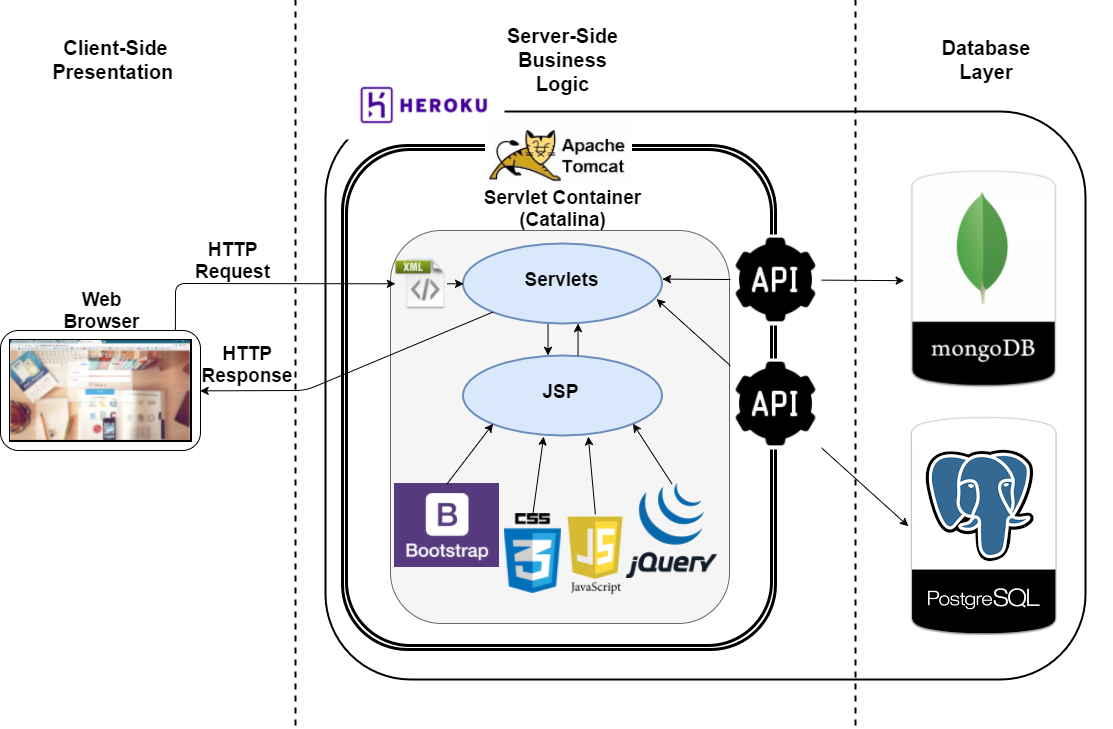
\includegraphics[width=13cm, height=9cm]{img/Architecture}
\caption{System Architecture.}
\end{figure}

\section{System Backend}
The backend manages all the data that is being consumed by the frontend
(JSP).The backend consists of three major components: Databases, Servlets and Security.

\subsection{Databases}
We chose to use two databases to store our data, that being MLab MongoDB and PostgreSQL. Both of these databases are being hosted online on Heroku. MLab was founded in 2011 and provides a fully managed cloud database service that can host MongoDB databases. Heroku offers a free plan for MLab MongoDB with up to 500MB free storage with paid plans thereafter. The purpose of MongoDB is to store the users data eg. Timetable and Calendar. There are six collections in the database, each to store a different set of data for the web application.

\begin{figure}[h]
\centering
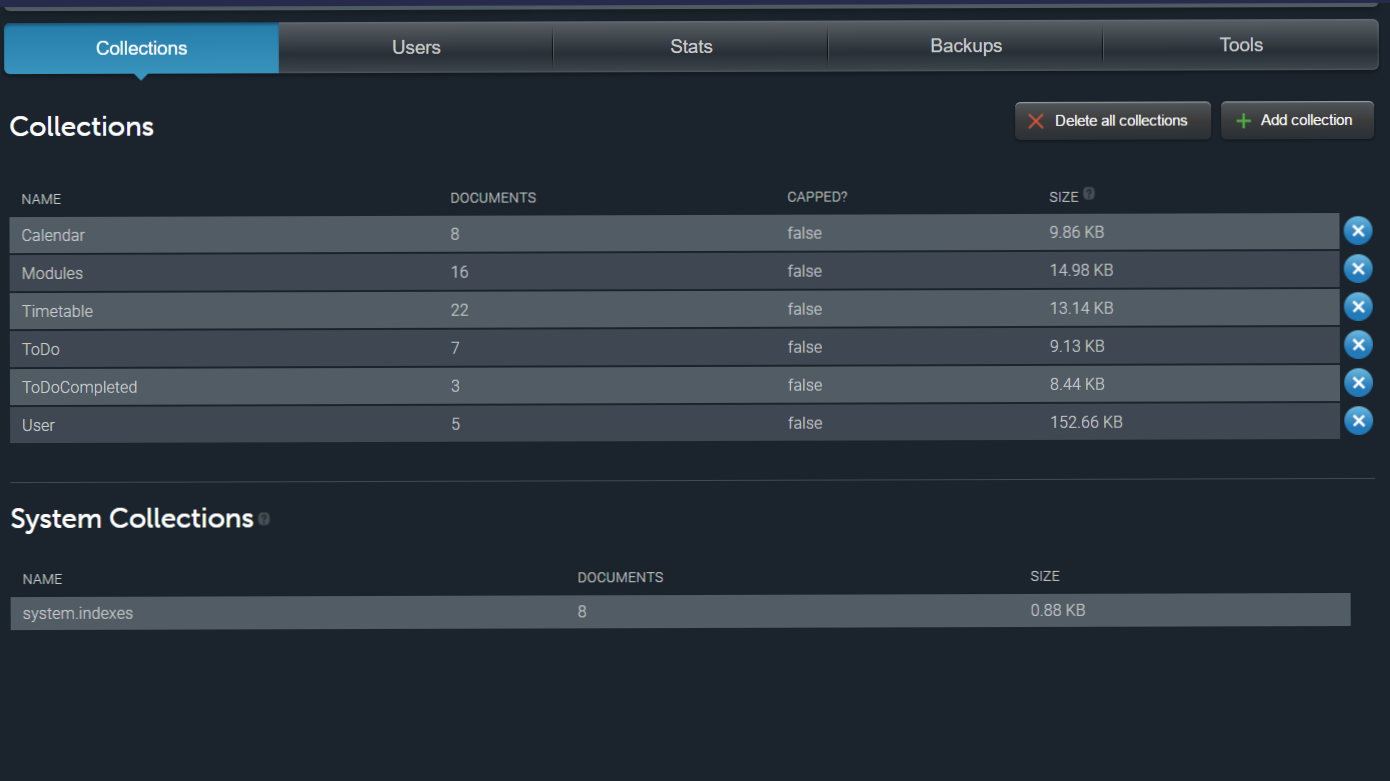
\includegraphics[width=15cm, height=10cm]{img/MongoDB}
\caption{MLab MongoDB Collections.}
\label{fig:MongoDBCollections}
\end{figure}

MongoDB stores data in flexible, JSON-like documents, meaning fields can vary from document to document and data structure can be changed over time\cite{MongoAbout}. Each collection has a different structure with Modules Collection being the most complex.  Below is a sample of a database entry from the Modules collection.
\begin{minted}{json}
{
    "_id": {
        "$oid": "58d1725bca932f463063d4a2"
    },
    "Confirmation Code": "rb5vnu4iqo0d13aqi2558qlv5j",
    "Title": "Artificial Intelligence",
    "Lecturer": "John Healy",
    "Grades": [
        {
            "ModuleTitle": "Artificial Intelligence",
            "Title": "CA",
            "Date": "2017-03-09",
            "Value": "20",
            "Result": "90"
        },
        {
            "ModuleTitle": "Artificial Intelligence",
            "Title": "CA 2",
            "Date": "2017-03-24",
            "Value": "30",
            "Result": "78"
        }
    ],
    "Assignments": [
        {
            "ModuleTitle": "Artificial Intelligence",
            "Title": "Maze Game",
            "Date": "21/04/2017",
            "Value": "50"
        }
    ]
}

\end{minted}

To communicate with the MongoDB data we use the MongoDB Java Driver API which provides both synchronous and asynchronous interaction with MongoDB\cite{JavaMongoDriver}. A single class named MongoConnection handles all the incoming and outgoing connections to the MongoDB database. The following code snippet is used to pull data from MongoDB and display in the web application:


\begin{minted}{java}
/**
 * getModuleGrades() returns a list of Grades
 * from each Module in the database.
 * 
 * @param code
 * @return list of Grades
 */
  public List getModuleGrades(String code) {
    List moduleGradesList = new ArrayList<>();
    MongoClientURI uri = new MongoClientURI(mongoAddress);
    MongoClient client = new MongoClient(uri);
    DB db = client.getDB(uri.getDatabase());
    DBCollection user = db.getCollection("Modules");
    BasicDBObject query = new BasicDBObject();
    query.put("Confirmation Code", code);

    BasicDBObject fields = new BasicDBObject("Grades",1).append("_id",false);
    DBCursor cursor = user.find(query, fields);
    if(cursor.hasNext()) {
      for (DBObject dbObject : cursor) {
      BasicDBList grades = (BasicDBList) dbObject.get("Grades");
      BasicDBObject[] gradeArr = grades.toArray(new BasicDBObject[0]);
      for(BasicDBObject dbObj : gradeArr) {
        String title = (String) dbObj.get("ModuleTitle");
        String gradeTitle = (String) dbObj.get("Title");
        String Date = (String) dbObj.get("Date");
        String Value = (String) dbObj.get("Value");
        String Result = (String) dbObj.get("Result");
        String s[] = new String[6];
        s[0] = title;
        s[1] = gradeTitle;
        s[2] = Date;
        s[3] = Value;
        s[4] = Result;
        moduleGradesList.add(s);
        }
      }
    }
  client.close();
  return moduleGradesList;
}
\end{minted}

PostgreSQL is an object-relational database management system that supports a large part of the SQL standard. We chose Heroku's free Hobby Dev plan for our web application but there are paid plans that offer extensive benefits. The purpose of postgreSQL is the store user accounts, which includes all the users details from their username to their biography. Each use is given an authentication cod when the register, which is stored along with their account in the database. The following is an example of a query on the database along with the query results.

\begin{figure}[h]
\centering
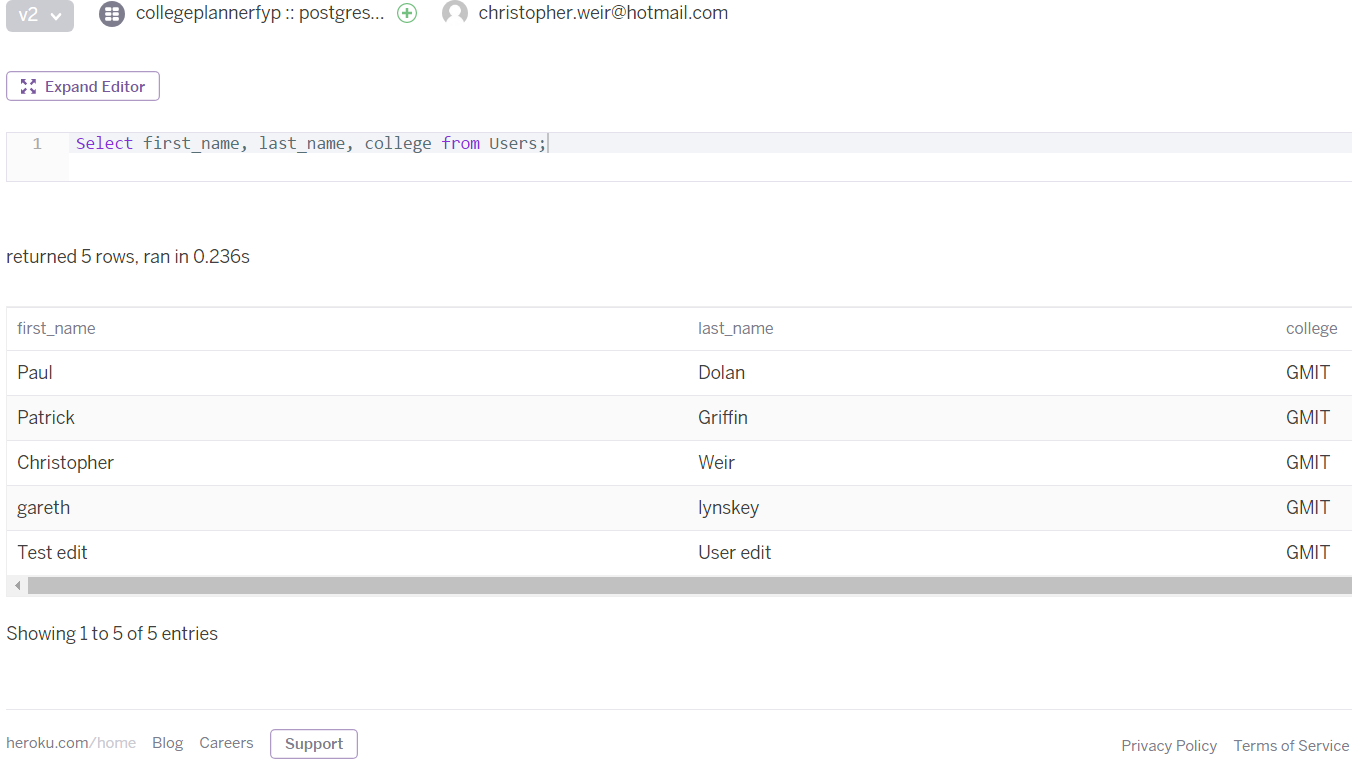
\includegraphics[width=15cm, height=10cm]{img/SQL}
\caption{PostgreSQL Query Sample.}
\end{figure}

To query the database from Java, we used the PostgreSQL JDBC API which allows us to communicate with the database. A single class named SQLConnection handles all of the incoming and outgoing communication to the database. To establish the connection with the database we used the following code snippet:

\begin{minted}{java}
/**
  * getConnection() gets the connection to the database.
  * 
  * @return the connection
  * @throws URISyntaxException
  * @throws SQLException
  * @throws ClassNotFoundException
*/
  public Connection getConnection() throws URISyntaxException,
                          SQLException, ClassNotFoundException {
    //Establish a connection with the database
    Class.forName("org.postgresql.Driver");
    String ConnectionString ="jdbc:postgresql://ec2-54-75-239-190.
    eu-west-1.compute.amazonaws.com:5432/dc6f77btle9oe3?user=dmble
    akzbhlbnl&password=b08ab093aa5b03c4047c541ceab2b23daa4fb5198e4
    8d56f804319695455d754&ssl=true&sslfactory=org.postgresql.ssl
    .NonValidatingFactory";
    return DriverManager.getConnection(ConnectionString);
  }
\end{minted}

Below is another code snippet that demonstrates a query from java to the postgreSQL database.

\begin{minted}{java}
/**
  * updateUserDetails() edits user details on the database.
  * 
  * @param userDetails
  * @throws SQLException
  * @throws ClassNotFoundException
  * @throws URISyntaxException
*/
    public void updateUserDetails(UserDetails userDetails) 
        throws SQLException, ClassNotFoundException, URISyntaxException{
    //Establish a connection with the database
    Connection connection = getConnection();

    //Create a new PreparedStatement
    PreparedStatement update = connection.prepareStatement
    ("UPDATE Users SET first_name =?, last_name =?,
        email =?, college =?, course =?, bio =? 
        WHERE confirmation_code =?");
    update.setString(1, userDetails.getFirstName());
    update.setString(2, userDetails.getLastName());
    update.setString(3, userDetails.getEmail());
    update.setString(4, userDetails.getCollege());
    update.setString(5, userDetails.getCourse());
    update.setString(6, userDetails.getBio());
    update.setString(7, userDetails.getCode());
    update.executeUpdate();
    
    connection.close();
    }
	
\end{minted}

\subsection{Servlets}
The JEE Servlets handle all the requests to the web application, and delegate all the appropriate responses back to the client. Each Servlet class is mapped using xml to a specific URL as shown below.

\begin{minted}{xml}
<servlet>
    <display-name>Profile</display-name>
    <servlet-name>Profile</servlet-name>
    <servlet-class>ie.gmit.sw.Profile.Profile</servlet-class>
</servlet>
<servlet-mapping>
    <servlet-name>Profile</servlet-name>
    <url-pattern>/Profile</url-pattern>
</servlet-mapping>	
\end{minted}

There are nine sections to the web application in total with each section having its own servlet which will be briefly explained below.\\

\par The \textbf{Login Servlet} is responsible for allowing the user to log in to the web application by first retrieving the username and password that was entered on the Login/Register page. The doPost() method then establishes a connection with the postgreSQL database on Heroku. A database query is made to check if the user exists and if it does then check if the password matches the users password. Once confirmed, the users data is passed into the request object and forwarded to the Profile page.\\

\par The \textbf{Register Servlet} is responsible for allowing the user to register an account on the web application. The doPost() first retrieves the details that were submitted by the user and then invokes a method in the SQLConnection class to query the postgrSQL database to check if the username or the email already exists. If either exist then an error is returned to the user informing them of this. If neither exist then the users details are added to the database and the users MongoDB entry will be created. The user is then redirected back to the Login/Register page.\\

\par The \textbf{Account Recovery Servlet} handles the recovery of user accounts. First the doGet() is called which sends the AccountRevovery jsp back to the client. The doPost() retrieves the username and email address that the user entered on the jsp form. These details are then sent to the postgreSQL database to be checked. If they belong to the same account the doPost() loads the RecoverAccount page to allow the password to be reset. The doPost() retrieves the new password entereed and applies it to the account. The user is then redirected back to the Login/Register page.\\

\par The \textbf{Profile Servlet} is responsible for retrieving the users profile from the postgreSQL and MongoDB database, handling profile editing and the removal of profiles. When the servlet is called the doGet() queries both databases based upon a code in the session. This code is known as an authentication code. Every user is assigned a unique code upon creation of their account. It is the "key" used to connect both database to a specific user. The doGet() passes the data from the database to the jsp which is then sent in the response to the user. When the user is editing their account, the doPost() retrieves the necessary inputted information from the jsp form and sends the edited details to the databases. However, if the user wishes to delete their account, the doPost() will check if the password entered matches their account password. If they match then the users account will be deleted from both databases. If it does not match the user is notified of this.\\

\par The \textbf{Calendar Servlet} dynamically displays the users calendar events on the jsp. The doGet() does this by first querying the MongoDB database through the MongoConnection class based upon the users code, which returns a list of calendar events. This list is outputted as Json by using Gson, to the jsp page. The doPost() handles all of the new event that are created, the editing of current events, and the deletion of current events. The doPost() retrieves the form data from the jsp and sends it to the MongoConnection class to be added to the database.\\

\par The \textbf{Timetable Servlet} processes all the inputs and outputs, to and from the Timetable page. When creating a new entry on the timetable, the inputted data on the JSP form is passed into the servlets doPost() method which sends it to the MongoConnection class to be stored on the database. When retrieving the timetable, the servlets doGet() calls the appropriate method on the MongoConnection class which returns the list of modules from the timetable collection on the database. Each object in the list is passed one by one into a timetable object, which is then in turn set as an attribute on the session. That attribute is then invoked and iterated through on the JSP to display the data.\\

\par The \textbf{ToDoList Servlet} when called upon, loads the users ToDo list from the database through the doGet() method. The doGet() also retrieves the ToDo list that is completed from the database. These lists are then added to the sessions attributes to be invoked and iterated through on the JSP to display the data. The doPost() method is responsible for changes to these list whether new entries are added, entries are moved from one list to the other, or entries are deleted entirely. These entries are again retrieved and sent to the MongoConnection class to be added, moved, or delete from the database.\\

\par The \textbf{Modules Servlet} is responsible for retrieving the users modules from the MongoDB database, calculating the users module total and overall GPA, adding new modules and results to the database, and removal of both module results and modules from the database. The doGet() handles the retrieval of modules along with the calculations, it also sends the jsp in the response to the user with the database data attached as session attributes. The doPost() handles the retrieval and sending of new modules, module results, deleted modules and deleted module results to the database. Again, the doPost() does this by retrieving the data from the jsp forms and sends it to the MongoConnection class, which will in turn make the changes to the database.\\

\par The \textbf{Assignments Servlet} is almost identical to the Modules Servlet, however it only focuses on the module assignments. The doGet() when called queries the MongoDb database to retrieve the users modules and their assignments. Both the modules and their assignmets are individually attached as session attributes. These attributes are then invoked by the Assignments jsp when sent to the user as the response. New assignments and the removal of assignments are handled by the doPost() method, which first retrieve the assignment to be added or removed and passes them along to the MongoConnection class to be added or removed from the database.\\

\par The following is an example of the Login Servlet:

\begin{minted}{java}
package ie.gmit.sw.Login;
import java.io.IOException;
import javax.servlet.*;
import ie.gmit.sw.Connections.SQLConnection;
import ie.gmit.sw.Security.Encryption;

public class Login extends HttpServlet{
  private static final long serialVersionUID = 1L;
  private LoginValues login = new LoginValues();
  private SQLConnection sqlConn = new SQLConnection();
  private Encryption encrypt = new Encryption();
  
  protected void doGet(HttpServletRequest request, 
                        HttpServletResponse response) 
                        throws ServletException, IOException
  {
    RequestDispatcher rd = request.getRequestDispatcher("LoginRegister.jsp");
    rd.forward(request, response);
  }
  protected void doPost(HttpServletRequest request,
                         HttpServletResponse response)
                         throws ServletException, IOException 
  {
    try{
      login.setUsername(request.getParameter("username"));
      login.setPassword(encrypt.encrypt((request.getParameter("password"))));
      sqlConn.userLogin(login);
      if(login.getPass() != null{
        if(login.getPass().equals(login.getPassword())){
          HttpSession session = request.getSession();
          session.setAttribute("firstname", login.getFirstname());
          session.setAttribute("lastname", login.getLastname());
          session.setAttribute("email", login.getEmail());
          session.setAttribute("college", login.getCollege());
          session.setAttribute("username", login.getUser());
          session.setAttribute("course", login.getCourse());
          session.setAttribute("bio", login.getBio());
          session.setAttribute("code", login.getCode());
          response.sendRedirect("Profile");
        }
        else{
          request.setAttribute("error","Invalid Username or Password");
          doGet(request, response);
        }
      }
      else{
        request.setAttribute("error","Invalid Username or Password");
        doGet(request, response);
      }
    }catch (Exception e) {
      response.sendRedirect("ErrorHandler");
    }
  }
}
\end{minted}

\subsection{Security}
The Web Applications security is managed by an Authentication Filter and data encryption. The Authentication Filter is mapped to the web application through the following XML code snippet:

\begin{minted}{xml}
<filter>
    <filter-name>AuthenticationFilter</filter-name>
    <filter-class>ie.gmit.sw.Security.AuthenticationFilter</filter-class>
</filter>
<filter-mapping>
    <filter-name>AuthenticationFilter</filter-name>
    <url-pattern>/*</url-pattern>
</filter-mapping>
\end{minted}
It restricts access to the web application if a user is not logged in by only allowing them to access the Login/Register page. When a user is logged in their unique authentication code get stored in the session, this allows the user to access the full web application. When they log out their code is removed from the session which activates the filter once again.\\

\par The users passwords are encrypted using SHA-512 with Salt which ensures the users data is secure. SHA-512 is one of several cryptographic hash functions. We use Salt with SHA-512 to further secure our users' passwords. Based upon this, it would take a brute force decryption algorithm running at 1 billion keys per second around 2788548552832941600 years 78 days 15 hours 56 minutes and 38 seconds or 3 quintillion years to break the password encryption.

\section{Front End (JSP)}


\begin{minted}{jsp}
<%@ page language="java" contentType="text/html; charset=ISO-8859-1"
	pageEncoding="ISO-8859-1"%>
<html>
  <body>
    <div class="form-group">
      <label>Module Title:</label>
      <input class="form-control" type="text" 
          id="moduleTitle" name="moduleTitle" 
          placeholder="Module Title max 30 characters" 
          maxlength="30">
      <!-- JSP file format -->
      <%
        String error_msg = (String) request.getAttribute("error");
        if (error_msg != null)
        out.println("<font color=red size=4px>" + error_msg + "</font>");
      %>
    </div>
  </body>
</html>
\end{minted}


\subsection{Login/Register}
\par The login page is the entering of information that identifies a user so that user is to have their own unique information. The login requires the user for the input of two pieces of information, a username and password. A username is a string that uniquely identifies the user and a password which is to be kept secret. The advantage of user login is it enables the web page to be personalized so the user can have its own information the way they want it. 
\begin{figure}[h]
\centering
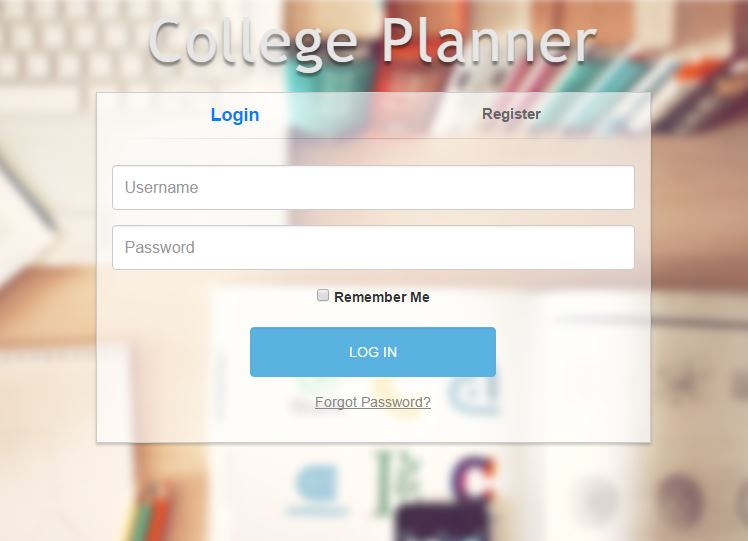
\includegraphics[width=8cm, height=6cm]{img/loginScreen}
\caption{Login Page}
\end{figure}
\newpage
\par If the user doesn’t have an account he/she can create one on the Register page. The user must enter the required details such as Username, First Name, Email, Password, and College. The user must also confirm their password so that they must match. If the user missed a credential they will be prompted to enter it.  When the user then registers, it’ll bring them to their profile page.
\begin{figure}[h]
\centering
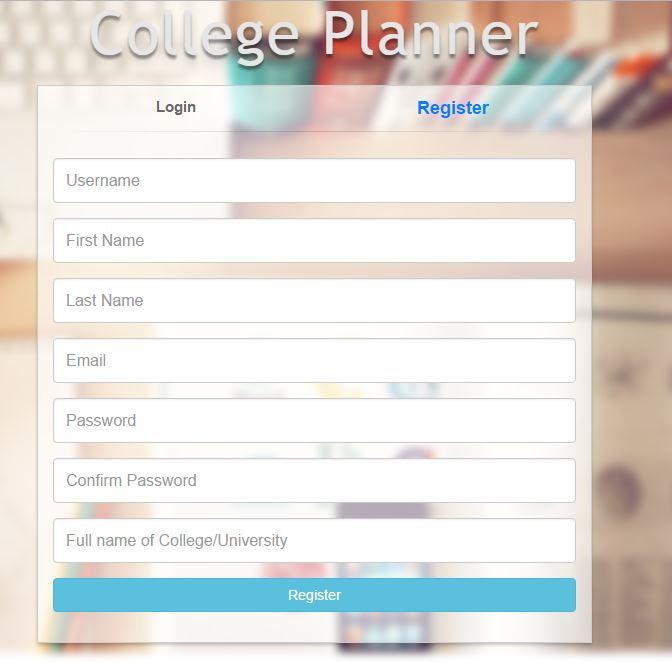
\includegraphics[width=8cm, height=7cm]{img/Registration}
\caption{Registration Page}
\end{figure}
\newpage
\subsection{Account Recovery}
The Account Recovery page is constructed from two JSP pages, the first being AccountRecovery and the second RecoverAccount. These pages are responsible for allowing the user to reset their account password if they have forgotten it. The user can navigate to this page from the Login/Register page. Upon navigating to these pages the user is first met with the AccountRecover jsp, here the user can enter their username and email address that is registered to the account that they wish to reset. These details are then passed to the PostgreSQL database to be checked. One condition allows for access to the RecoverAccount page and that is that the username and email entered must belong to the same account. If this condition is not met then the user will not be granted access and they will simply be return to the same page.

\begin{figure}[h]
\centering
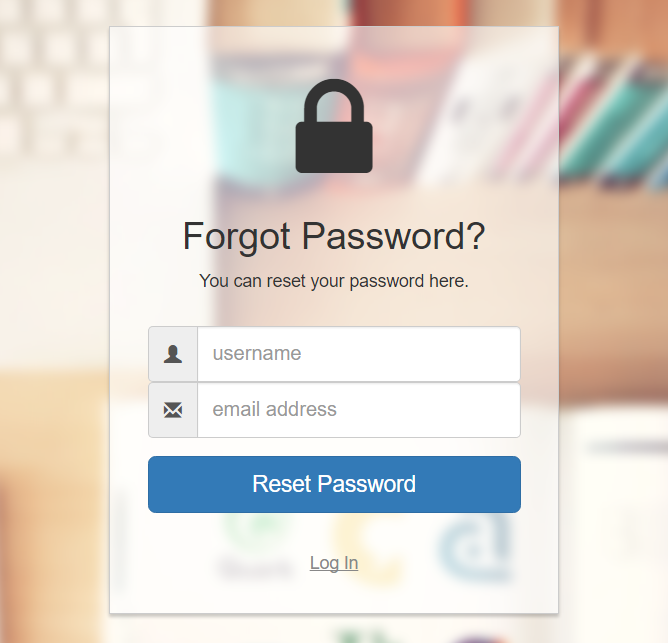
\includegraphics[width=8cm, height=7cm]{img/AccountRecovery}
\caption{AccountRecovery Page}
\label{fig:AccountRecovery}
\end{figure}

However, if the condition is met, the user will be redirected to the RecoverAccount page. Here the user will be able to enter a new password which will then be save to their account. The user will then be redirected to the Login/Register page.

\begin{figure}[h]
\centering
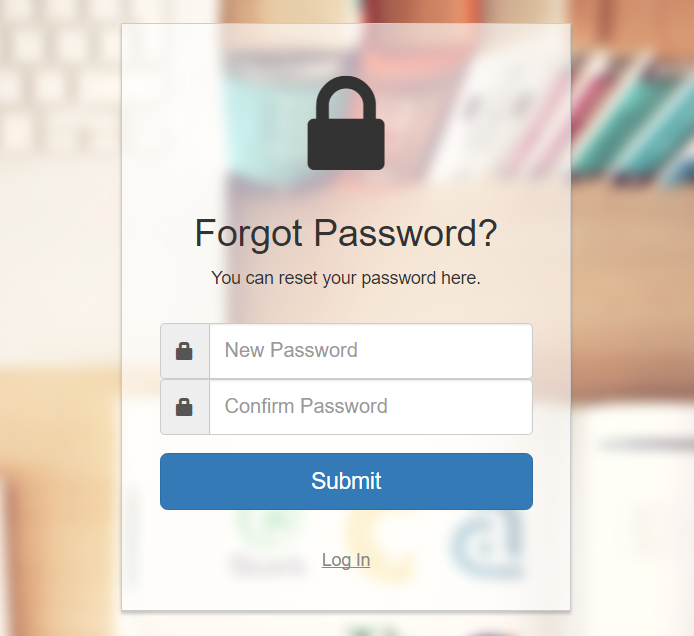
\includegraphics[width=8cm, height=7cm]{img/RecoverAccount}
\caption{RecoverAccount Page}
\label{fig:RecoverAccount}
\end{figure}
\newpage
\subsection{Profile}
After a successful login, the user is redirected to the Profile page. The Profile page contains the users account details, which can be edited and deleted. 

\begin{figure}[h]
\centering
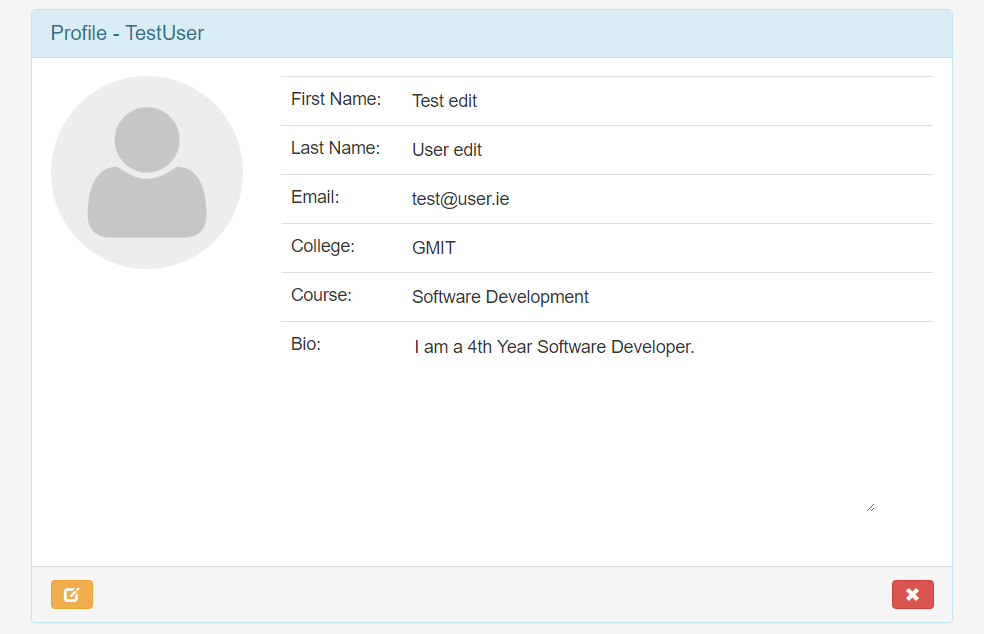
\includegraphics[width=9cm, height=6cm]{img/Profile}
\caption{Profile Page}
\label{fig:Profile}
\end{figure}

The details can be edited by first clicking the yellow edit button, the user can then change whatever they wish. The user will also find two extra details that they can chose to fill in, their course title and a bio section. A custom profile picture can also be uploaded by clicking on the edit button below the current profile picture. To save the new details or the profile picture, the user must click the green save button. 

\begin{figure}[h]
\centering
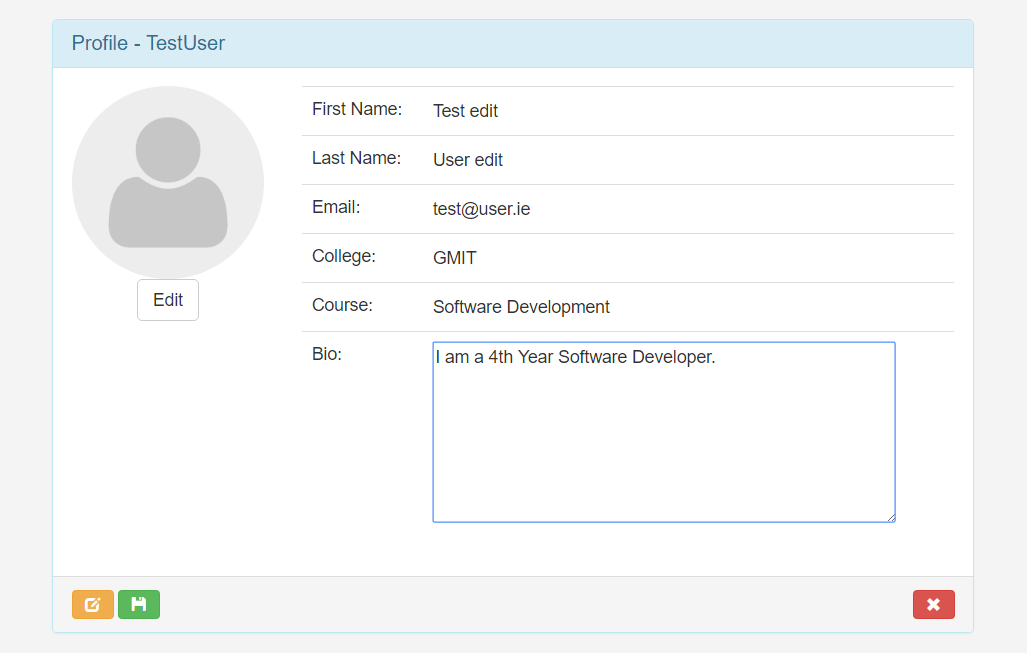
\includegraphics[width=9cm, height=7cm]{img/ProfileEdit}
\caption{Edit Profile}
\label{fig:ProfileEdit}
\end{figure}

There is a red delete button which allow a user to delete their account. However, a bootstrap modal will appear first prompting the user to enter their password to confirm that they are sure about deleting their account. By clicking on the delete button once their password is entered, will permanently delete the users account.

\begin{figure}[h]
\centering
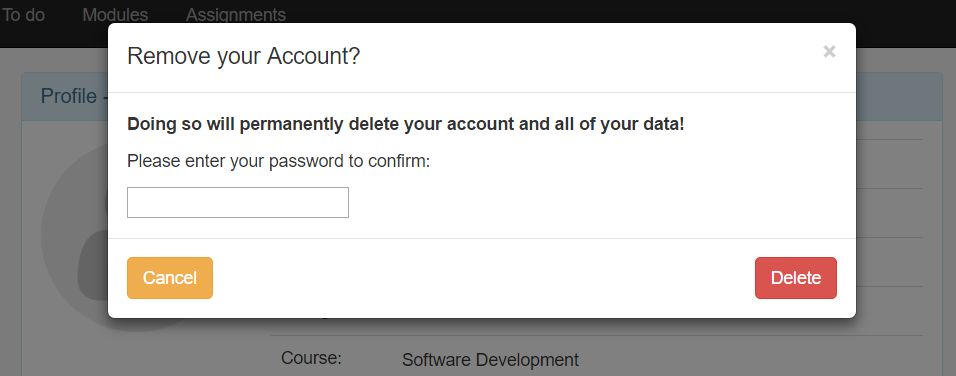
\includegraphics[width=10cm, height=5cm]{img/ProfileDelete}
\caption{Delete Profile}
\label{fig:ProfileDelete}
\end{figure}

\subsection{Calendar}
The Calendar page allows users to access a full calendar, week view and day view throughout the year. Users can also create events for a certain day or days depending on how long their event is. These events can be updated, deleted and edited. The events can also be color coded for better user experience. To create the Calendar, we implemented the FullCalendar library, which is a JavaScript event library that is fully customizable and is open source\cite{Calendar}. We used this library to display the calendar with the attributes that we wanted. We also linked the Assignments page and the Calendar so that when a User enters a Due Date for their Assignment it will popup on the Calendar on the date it was given.
\begin{minted}{js}

$(document).ready(function() {
 $('#calendar').fullCalendar({

 customButtons: {
  myCustomButton: {
   text: 'Create Event',
   click: function() {
    $("#myModal").modal();
   }
  }
 },

  header: {
   left: 'prev,next today myCustomButton',
    center: 'title',
    right: 'month,agendaWeek,agendaDay'
   },
   theme : false,
   editable : false,
   slotLabelFormat:"HH:mm",
   events : "CalendarEvents",
  }
});
\end{minted}
A custom button for the “create event” was added as seen in figure \ref{fig:create} that popups a bootstrap modal for the user to enter the required details. The events are passed from the Calendar page to its respective servlet, from here the event is sent to the MongoDB database. All Calendars and their events are stored on the Calendar collection on the database, which can be seen in figure \ref{fig:MongoDBCollections}. 
\begin{figure}[h]
\centering
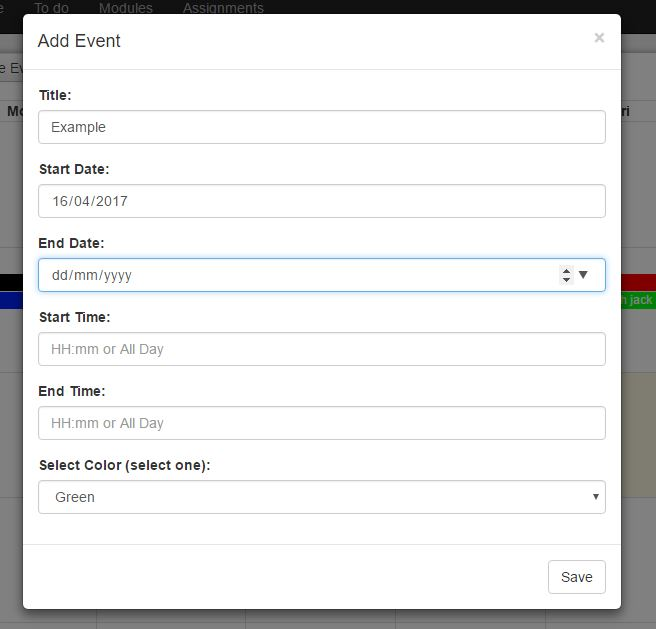
\includegraphics[width=8cm, height=7cm]{img/CalendarCreate}
\caption{Calendar Create event}
\label{fig:create}
\end{figure}
\newpage
\par
Then I’m using the Google GSON, a JSON library to convert the list of events data into a JSON feed from java objects\cite{Calendar}. I also set the content type as follows, which will specify what you are returning:
\begin{minted}{java}
response.setContentType("application/json");
response.setCharacterEncoding("UTF-8");
PrintWriter out = response.getWriter();

RequestDispatcher rg = request.getRequestDispatcher("Calendar");
out.write(new Gson().toJson(l));
\end{minted}
The above shows how to return a JSON object from a Java Servlet as it takes the printwriter object from response and to write the required JSON object to the object stream. UTF-8 is a character encoding capable of encoding all possible characters. This was necessary for populating the data onto the Calendar JSP page.

\begin{figure}[h]
\centering
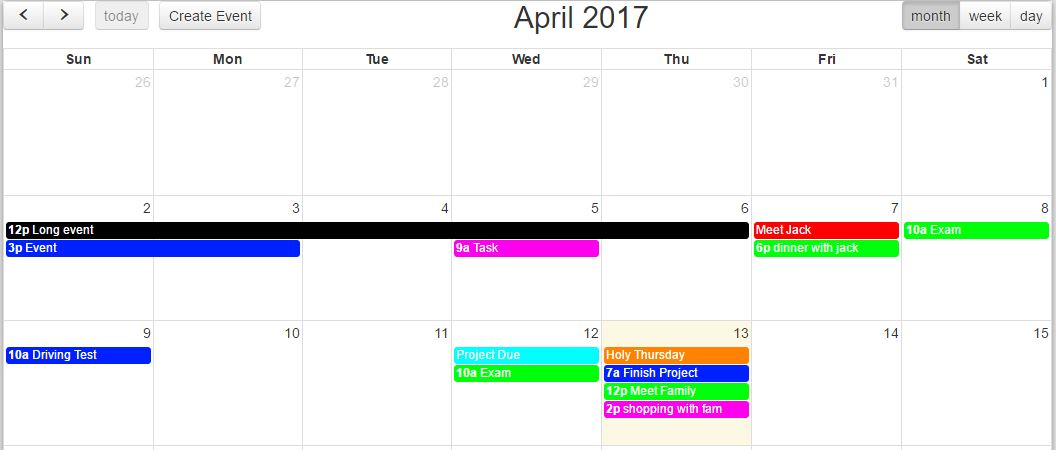
\includegraphics[width=11cm, height=6cm]{img/CalendarMonth}
\caption{Calendar Month View}
\label{fig:MonthView}
\end{figure}
\newpage
Figure \ref{fig:MonthView} is a full month view of events on multiple days or the same day. You will notice for certain events that numbers beside the events is the time it starts with ‘a’ or ‘p’ after indicating either am or pm so the user knows if it’s a morning event. You will also notice the “Project Due” event on the 12th which comes from the Assignments page so the user won’t have to create a separate event to remind the user.

\begin{figure}[h]
\centering
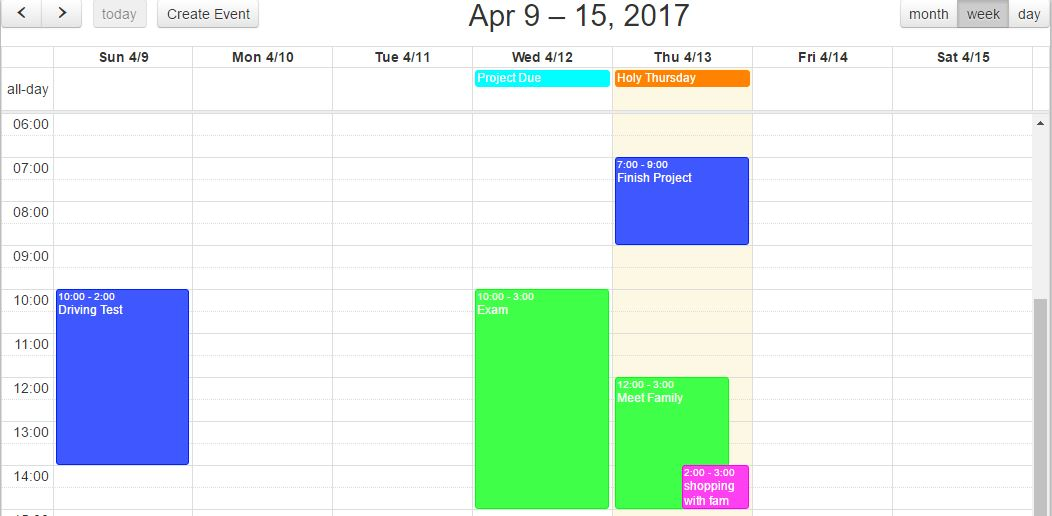
\includegraphics[width=10cm, height=6cm]{img/CalendarWeek}
\caption{Calendar Week View}
\label{fig:WeekView}
\end{figure}

Figure \ref{fig:WeekView} is the week view of events that shows a better view of the events for their allocated times. There is also a slot at the top for and event that’s “all-day”. These events are entered in from the user using a bootstrap modal where the user enters in the required details. I use JavaScript for error handling making sure that users enter valid information. 

\subsection{Timetable}
At the beginning of the development of the timetable, we adapted a tutorial found here\cite{Timetable}, which helped us understand the functionality required for a timetable to be implemented. This tutorial provided the basic foundation which we build upon ourselves. \par
The Timetable page allows users to create their own unique timetable for college. After navigating to the Timetable page, the first thing you will see is the timetable and an add module button above the timetable. The timetable should be empty unless it has been previously populated. We used the JSTL and Standard tag libraries to generate the timetable. 

\begin{minted}{jsp}
<%@ taglib uri="http://java.sun.com/jsp/jstl/core" prefix="c"%>
<html>
....
</html>
\end{minted}

The JavaServer Pages Standard Tag Library (JSTL) encapsulates as simple tags the core functionality to many Web applications. JSTL has support for structural tasks like iteration and conditionals, tags for manipulating XML documents, internationalization tags, and SQL tags. It also provides a framework for integrating existing custom tags with JSTL tags\cite{JSTL}. The standard tag library is always together with the JTSL tag library as it's used to enable the JTSL expression language in a JSP page.

\begin{figure}[h]
\centering
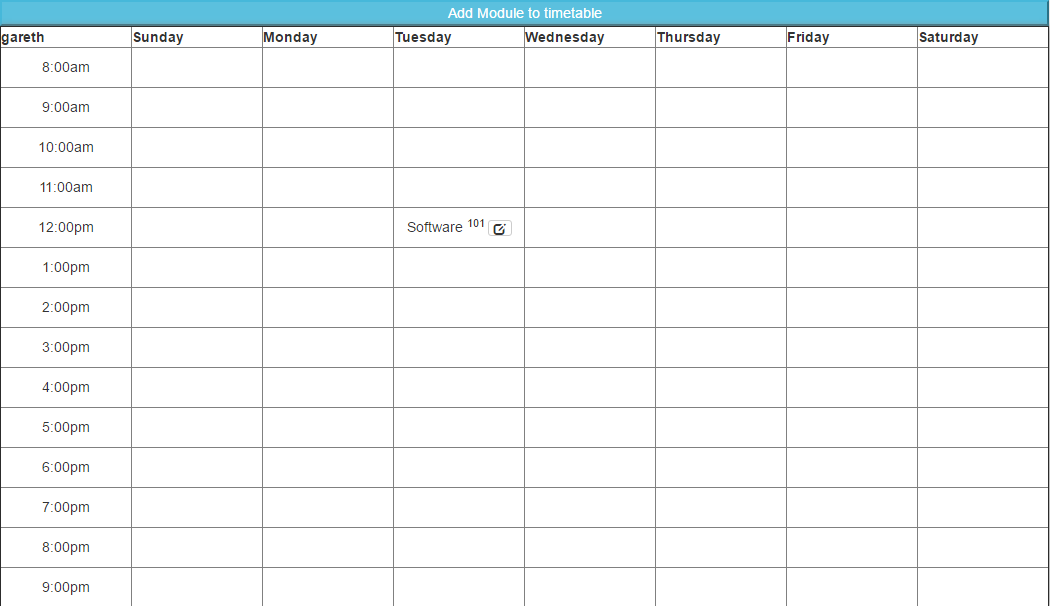
\includegraphics[width=12cm, height=6cm]{img/timetable}
\caption{Timetable}
\label{fig:timetable}
\end{figure}

The user is prompted to click the add module button to which a pop-up bootstrap modal will appear. The bootstrap pop-up modal is a form that contains all the required details of a module that must be entered to create a valid input for the timetable. The module title, room, start time, end time and day. When all the fields are filled out correctly, the user should click the add button and then the module will be added to the timetable and stored in the timetable collection in the Mongo database.

\begin{figure}[h]
\centering
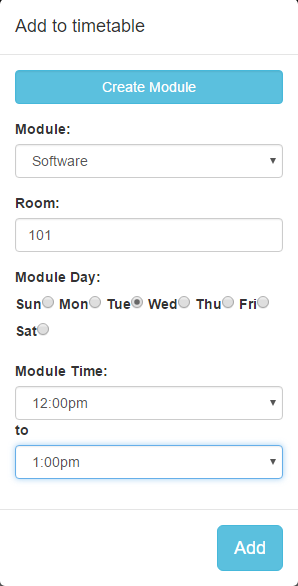
\includegraphics[width=5cm, height=8cm]{img/AddModule}
\caption{Add Module}
\label{fig:AddModule}
\end{figure}

When a module is visible on the timetable, there is an option to edit that module to the right of the module name. When the user clicks the edit button, a pop-up bootstrap modal will appear. On the bootstrap pop-up modal, the user is given the option to edit that modules data. At the bottom of the pop-up bootstrap modal, the user has the option to either save the changes made or delete the module from the timetable.

\begin{figure}[h]
\centering
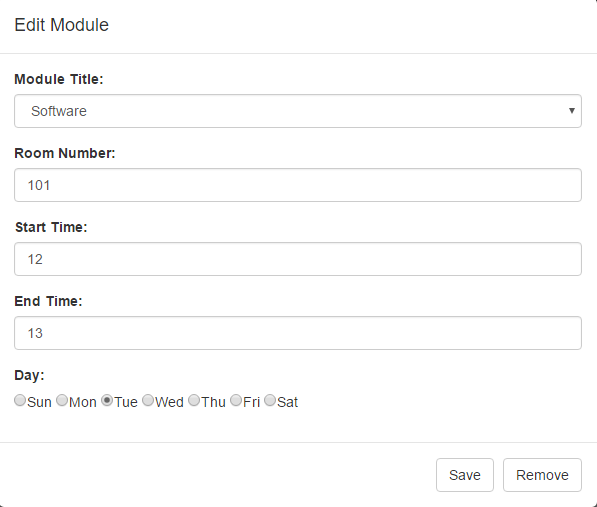
\includegraphics[width=10cm, height=10cm]{img/editModule}
\caption{Edit Module}
\label{fig:AddModule}
\end{figure}
\newpage
\subsection{To do List}
We wanted to keep the To-do simple and support the two main components of a normal to-do list which are add and delete. We also added other features where users can mark a task as done, where it then sends the task over to a task completed table. You can also transfer the task back to the to-do list table.

\par The To-do page is made up of two java classes along with a java servlet, JSP page and a connection to MongoDB. The user must first enter a title for a task followed by a description of the task with both fields required. When the user selects the save button, the task is sent to the To do List table and saved to that user’s profile on MongoDB.

\par When sent to the Todo List table, the task title is shown to the user and to view the description the user must click the description which then shows a pop up box of the description. For each task a check box is provided labelled ‘Mark as done’ and once the check box is selected the task is sent over to the Tasks Completed table so at that the user knows what tasks they have completed. The title of the task also has a line through it to show the user that the task is completed. We felt there was no need to display the description of the task once moved to the Tasks Completed table however if the user wishes to see the description of the task, all that has to be done is for the task to be transferred back to the To Do List table.  Once the task is sent to the Tasks Completed table, you then have the option of either transferring the task back to the Todo List table or deleting the task. This is in case users have accidentally sent the wrong task to the Tasks Completed table. Once the item is deleted from the Tasks Completed table it is then removed from the database. A bootstrap modal pop up box will appear when either the transfer or delete button is selected so as that the user does not delete the wrong task by accident. We used bootstrap and CSS to style the page, which makes it very user friendly for the user.

 


\begin{figure}[h]
\centering
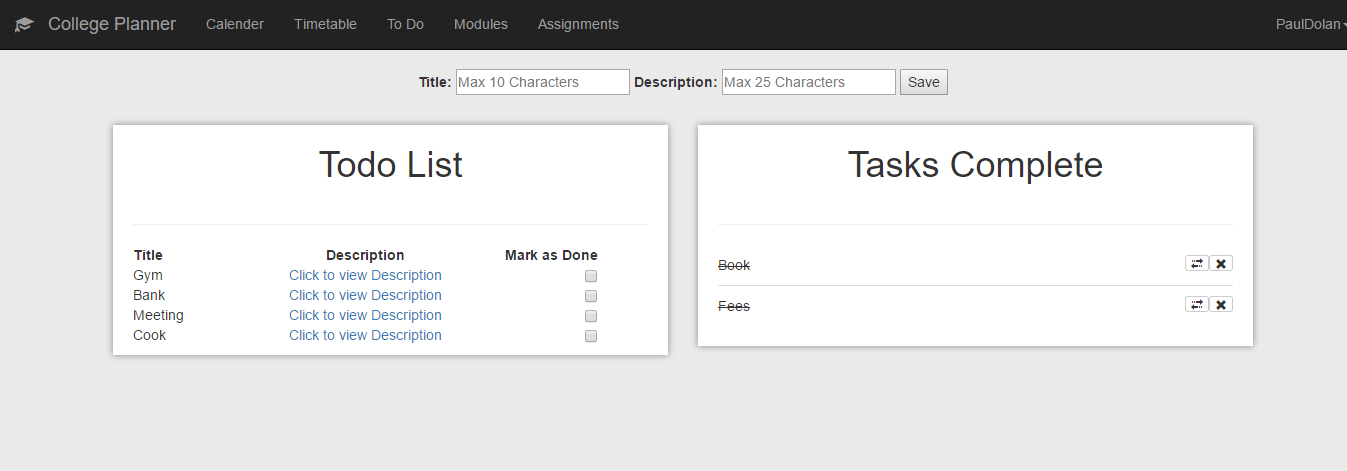
\includegraphics[width=13cm, height=5cm]{img/ToDo}
\caption{Todo Page}
\end{figure}


\subsection{Modules}
The Modules page was created as a way for users to keep track of their grades. After navigating to the Modules page, the user will see the title Modules, GPA, and a button. The user is prompted click the create module button to which a bootstrap pop-up modal will appear. The bootstrap pop-up modal is a form that contains the required fields that must be entered to create a valid module. The module title and lecturer.

\begin{figure}[h]
\centering
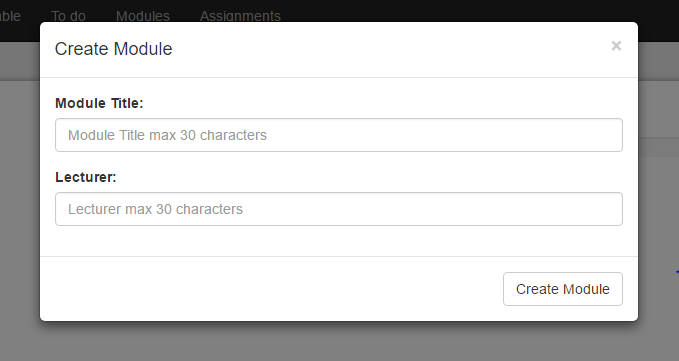
\includegraphics[width=10cm, height=7cm]{img/createModule}
\caption{Create Module}
\label{fig:CreateModule}
\end{figure}
\newpage
When all the fields are filled out correctly, the user should click the create module button and then the module will be displayed on the page and stored in the modules collection in the mongo database. The user has the option to delete the module to the right of the total percentage bar.

\begin{figure}[h]
\centering
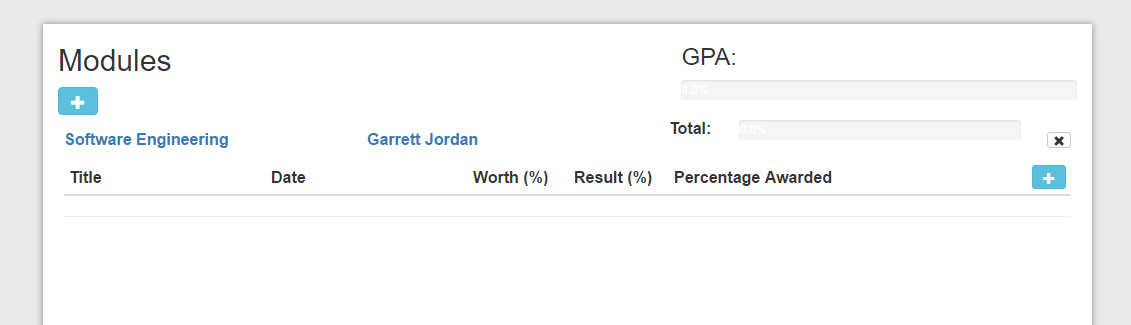
\includegraphics[width=10cm, height=3cm]{img/addedModule}
\caption{Modules}
\label{fig:Modules}
\end{figure}

After the module has been created, the user should click on the module and expand it. This will cause a table of empty fields to appear with the column names Title, Date, Worth (\%), Percentage (\%), Percentage Awarded, and an Add Grade button. When the user clicks the Add Grade button, a bootstrap pop-up modal will appear. The bootstrap pop-up modal contains the required fields that must be entered to create a valid grade entry to the module. The user should enter the grades title, date, what the percentage of the assessment or assignment is worth, and the percentage they received out of 100\%. 


\begin{figure}[h]
\centering
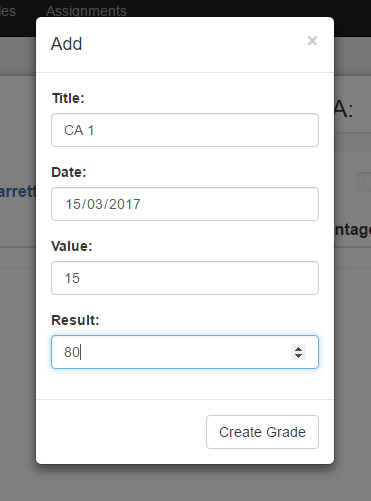
\includegraphics[width=6cm, height=6cm]{img/AddGrade}
\caption{Module Add Grade}
\label{fig:ModuleGrade}
\end{figure}
\newpage
When all the required fields are entered correctly, the user should click the Create Module button at the bottom of the bootstrap pop-up modal and it will populate the table. When the user expands the module it will display the result of that assessment or assignment, by calculating the percentage received out of what it was worth. The user has the option to delete the grade to the right of the percentage awarded. The user can add multiple modules and grades to them and at the top of the page, the total Grade Point Average (GPA) will be calculated.



\subsection{Assignments}
The Assignments page was created for the student to keep track of their upcoming due dates for projects, assignments or exams. The Assignments page is linked up with the Modules page so as that every module the student adds to the Modules page, will appear on the Assignments page. 

\begin{figure}[h]
\centering
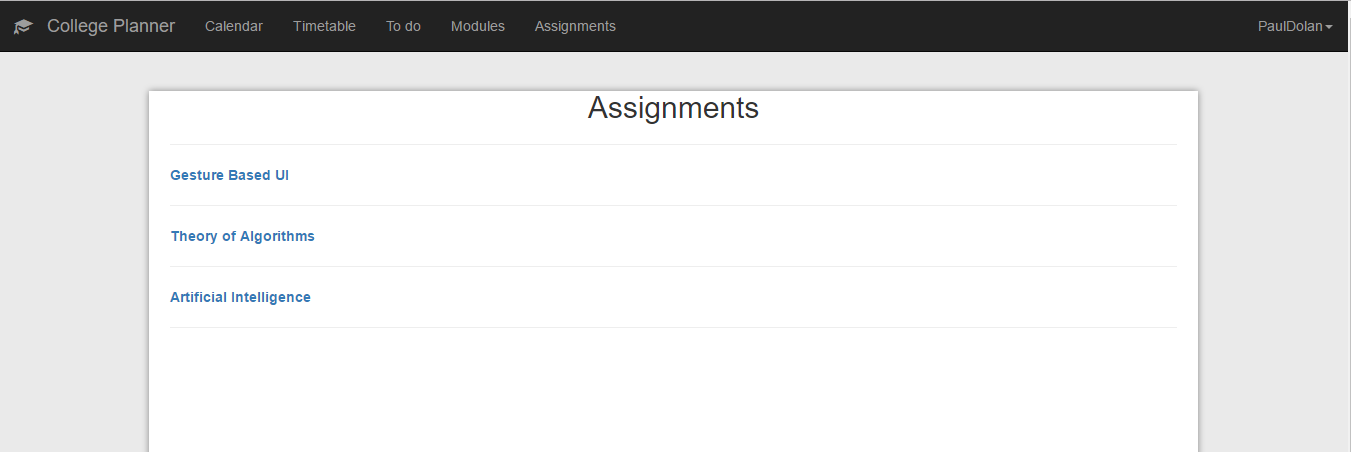
\includegraphics[width=11cm, height=4cm]{img/Assignments}
\caption{Assignments Page}
\end{figure}
\newpage
When the user selects one of the module names, they will then be shown whether they have any assignments due. If they have no assignments added into a module, the section will be empty. However if one or more assignments have been added, shown will be the title, the due date and how much the assignment is worth.

\begin{figure}[h]
\centering
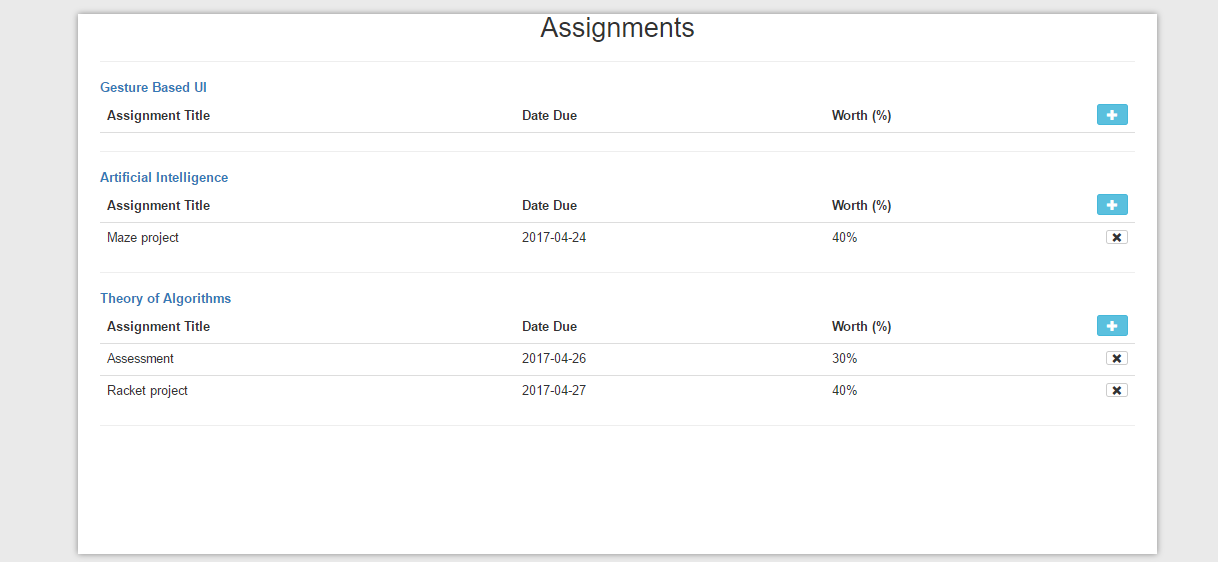
\includegraphics[width=11cm, height=5cm]{img/Assignments1}
\caption{Assignments Page Expanded}
\end{figure}

When the user wishes to add an assignment into a module, they must select add button provided. Once this button is clicked, a bootstrap pop up modal box will appear which must be filled in fully and correctly in order to create an assignment. The fields will prompt you for an assignment title, a due date and how much the given assignment is worth. Once you populate these required fields and create the assignment it will then be visible under the user’s module heading.

\begin{figure}[h]
\centering
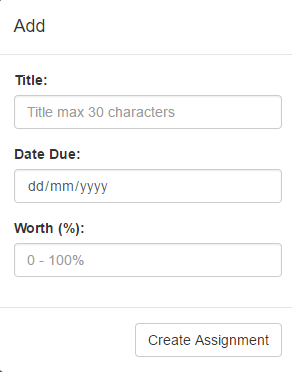
\includegraphics[width=7cm, height=9cm]{img/AddAssignment}
\caption{Assignments Page Modal}
\end{figure}
\newpage
Along with being linked to the Modules page, the Assignments page is also linked to the Calendar. This results in an event being created in the calendar for the given date on which the assignment was due. 


\subsection{Scripts and Styling}
The styling and scripting helped add design and functionality to the project. We mainly worked with bootstrap HTML templates for designing the look of our project. Below is an example of a Bootstrap that we used.

\begin{minted}{jsp}
<div class="modal fade" id="assignmentModal" role="dialog">
  <div class="modal-dialog modal-sm">
    <div class="modal-content ">
      <div class="modal-header">
        <h4 class="modal-title">Add</h4>
      </div>
      <div class="modal-body">
        <form id="createAssignment" action="Assignments" method="post">
          <div class="form-group">
            <label>Title:</label>
            <input class="form-control" type="text" 
            id="assignmentTitle" name="assignmentTitle" 
            placeholder="Title max 30 characters" maxlength="30">
          </div>
          <div class="form-group">
            <label>Date Due:</label>
            <input class="form-control" type="date" 
            id="assignmentDate" name="assignmentDate">
          </div>
          <div class="form-group">
            <label>Worth (%):</label>
            <input class="form-control" type="number" 
            id="assignmentValue" name="assignmentValue" 
            placeholder="0 - 100%" min="1"max="100">
          </div>
        </form>
      </div>
      <div class="modal-footer">
        <button form="createAssignment" name="submitBtn" 
        value="CreateAssignment" type="submit" 
        class="btn btn-default">Create Assignment</button>
      </div>
    </div>
  </div>
</div>
\end{minted}
To achieve the design aspects that we wished to incorporate into the web application, we used custom CSS to add these extra design features that Bootstrap could not provide. The following is a sample of the custom CSS:

\begin{minted}{CSS}
.title {
    font-size: 60px;
    font-family: Trebuchet MS;
    text-align: center;
    letter-spacing: 2px;
    text-overflow: ellipsis;
    text-shadow: 0px 4px 3px rgba(0, 0, 0, 0.4), 0px 8px 13px
    rgba(0, 0, 0, 0.1), 0px 18px 23px rgba(0, 0, 0, 0.1);
    color: rgb(230, 230, 230);
}

.panel-login {
border-radius: 0;
border-color: #ccc;
background-color: rgba(255, 255, 255, 0.6);
-webkit-box-shadow: 0px 2px 3px 0px rgba(0, 0, 0, 0.2);
-moz-box-shadow: 0px 2px 3px 0px rgba(0, 0, 0, 0.2);
box-shadow: 0px 2px 3px 0px rgba(0, 0, 0, 0.2);
}
\end{minted}

We used JQuery for the manipulation of elements on the JSP and for error handling as shown below.
\begin{minted}{js}
$('document').ready(function() {
    document.getElementById("imgPath").value=
      document.getElementById("image").src;
	
    updateData();
    function updateData() {
        document.getElementById("firstname").value =
        document.getElementById("fname").value;
        document.getElementById("lastname").value =
        document.getElementById("lname").value;
        document.getElementById("email").value =
        document.getElementById("em").value;
        document.getElementById("college").value =
        document.getElementById("coll").value;
        document.getElementById("course").value =
        document.getElementById("cour").value;
        document.getElementById("bio").value =
        document.getElementById("biog").value;
    }
    $(document).on("change, keyup", "#fname, #lname,
    #em, #coll, #cour, #biog", updateData);
    }
);

\end{minted}
However in situations where we could not use JQuery to handle these tasks, we used custom JavaScript.

\begin{minted}{JavaScript}
function editCheckTime(){
    var startTime = parseInt(document.getElementById("editStartTime").value);
    var endTime = parseInt(document.getElementById("editEndTime").value);
    
    if(startTime >= endTime){
        document.getElementById("errorEditTime").style.display = "block";
        return false;
    }
    else{
        document.getElementById("errorEditTime").style.display = "none";
        return true;
    }
    return false;
};
\end{minted}

\section{UML}
The following is a UML diagram to provide a visual representation of the web applications Java classes:

\begin{figure}[h]
\centering
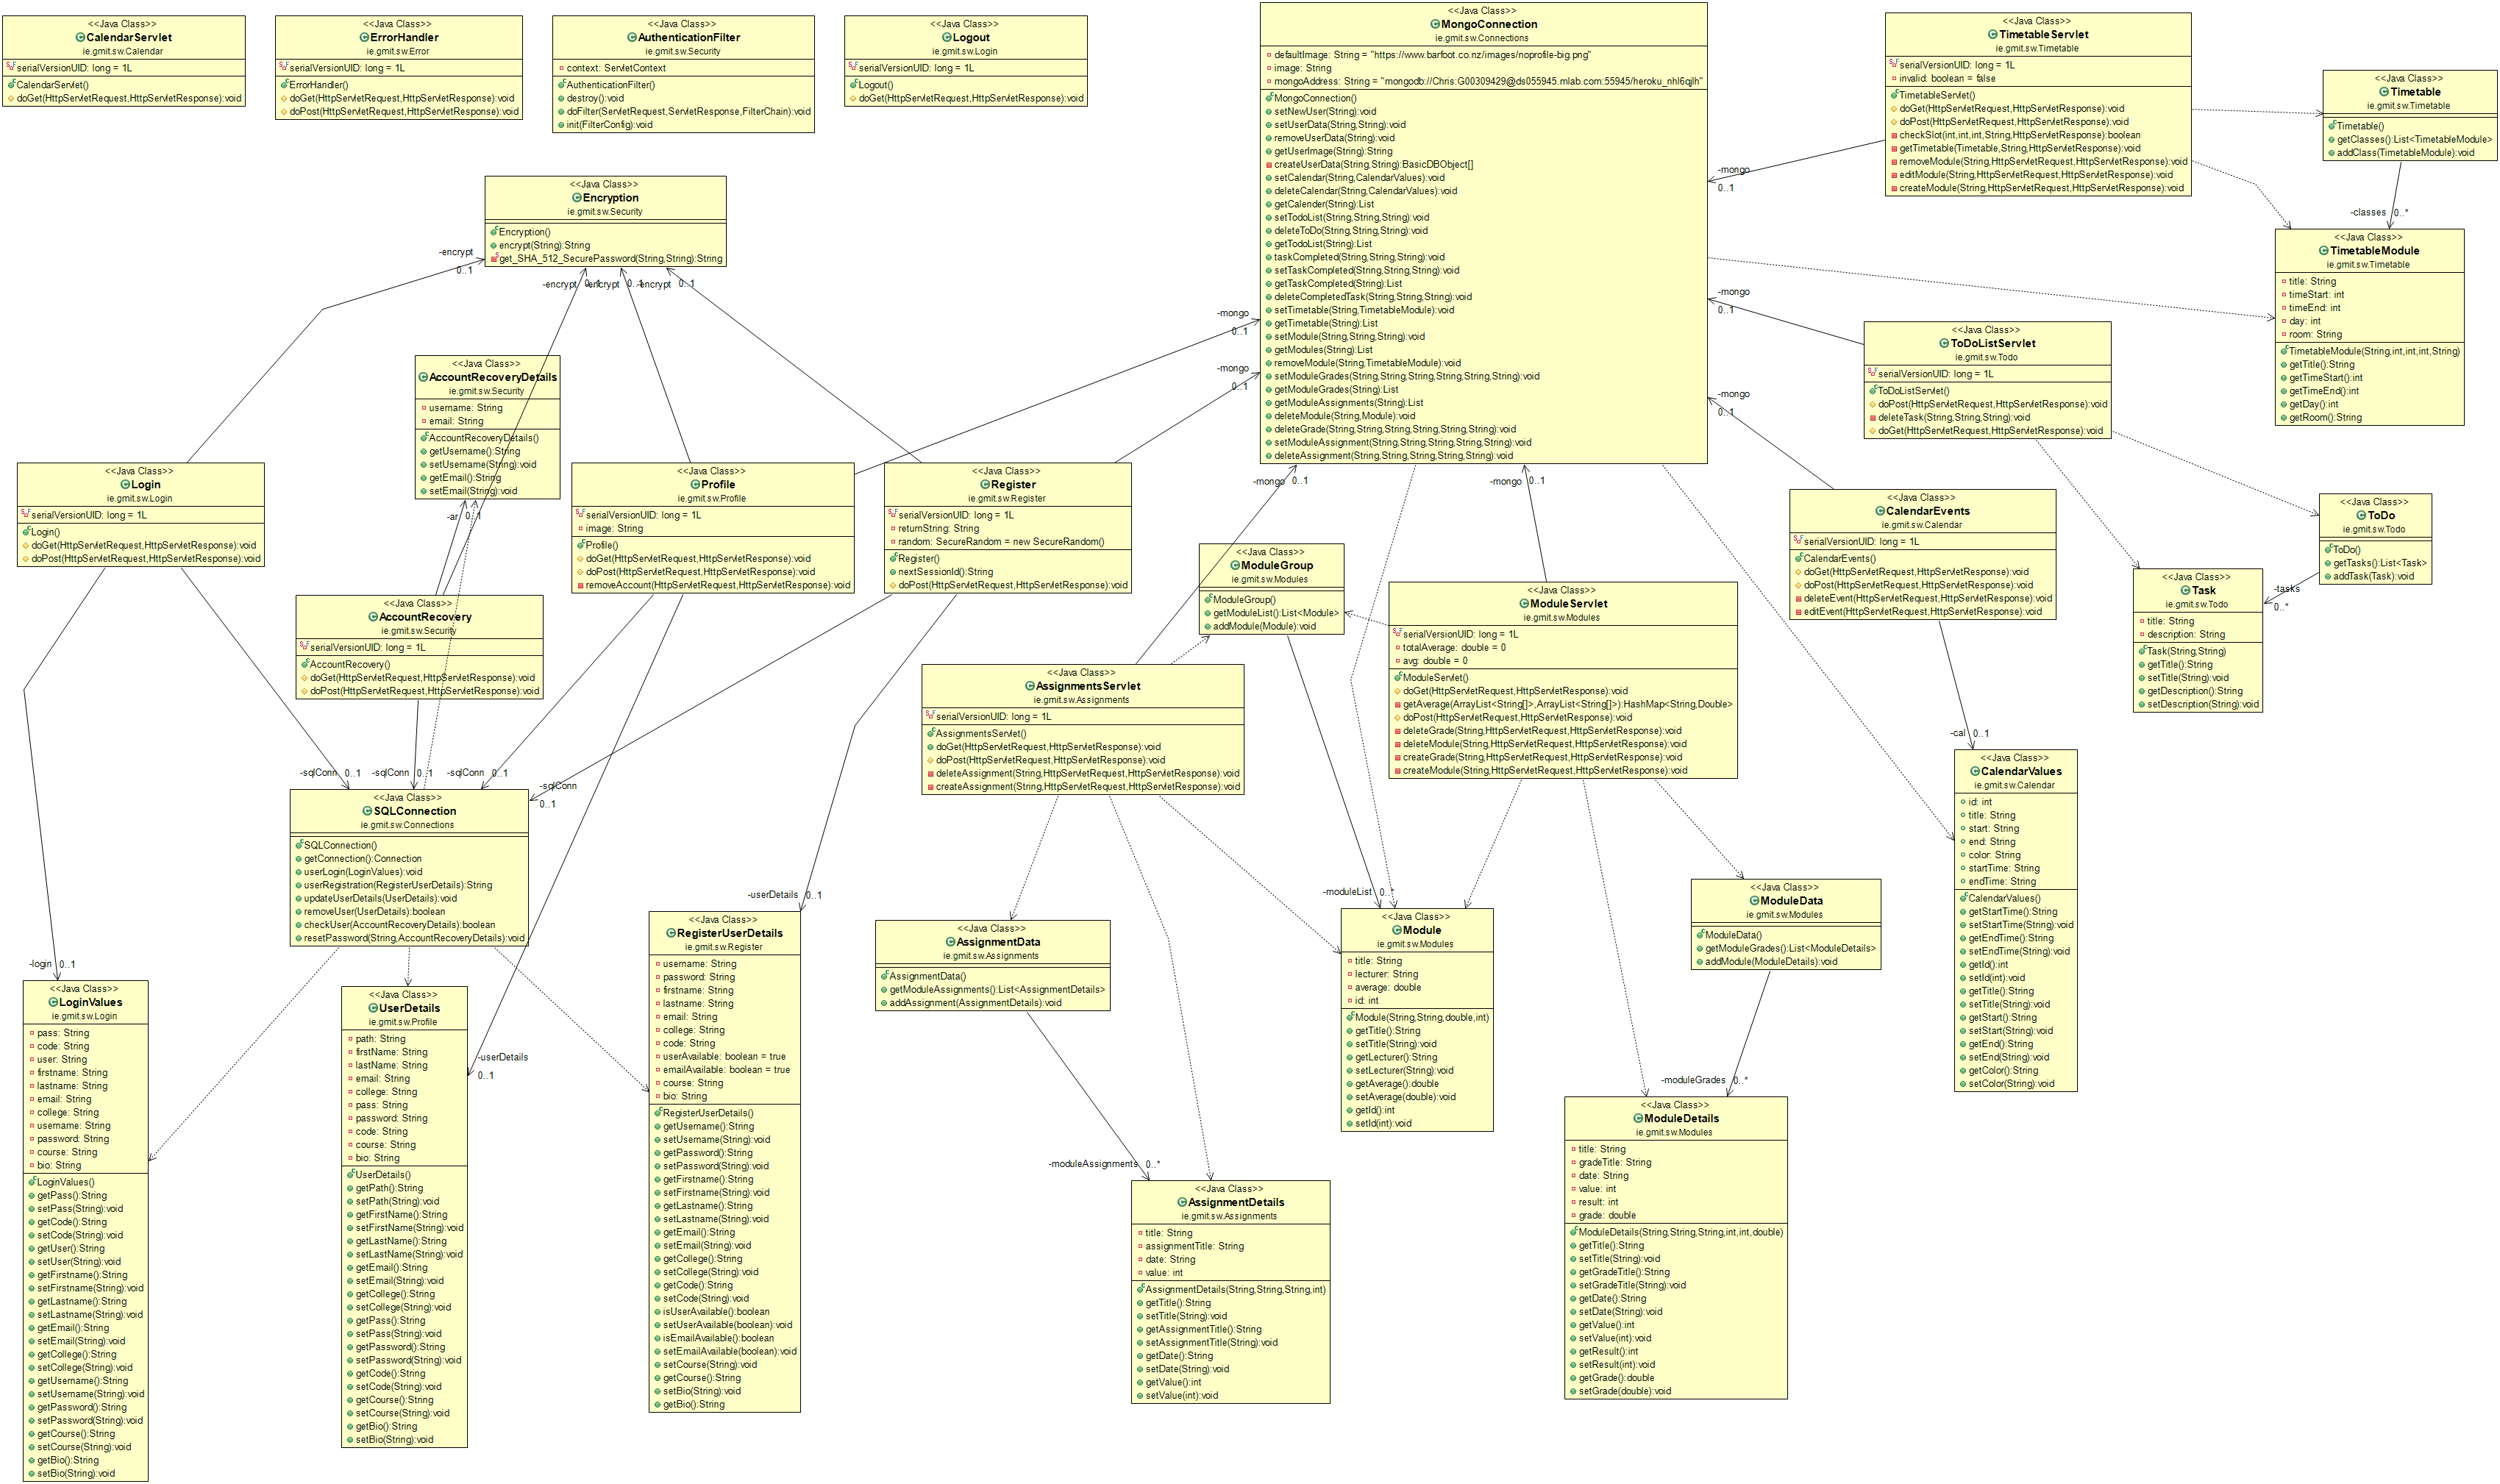
\includegraphics[width=12cm, height=7cm]{img/UML}
\caption{UML Diagram}
\end{figure}

\section{Deployment}
To deploy our web application onto Heroku we used the Heroku Command Line Interface (CLI). Heroku CLI allowed us to manage our application and configure our add-ons from the command line. Our project was exported from eclipse as a war file which we then used in the following command to upload the application to Heroku:

\begin{minted}{bash}
heroku war:
    deploy C:\Users\Chris\workspace\Final-Year-Project\CollegePlanner.war 
        --app collegeplannerfyp
\end{minted}

This command generates all the necessary files, from the war file, for Heroku to use to deploy the web application successfully.

\chapter{System Evaluation}
In this section, we are going to evaluate our web application based on different attributes. They are as follows:
\begin{itemize}
    \item Scalability
    \item Robustness
    \item Maintainability
    \item Extensibility
\end{itemize}

\par \textbf{Scalability:} The web application is highly scalable when the requirement grows or the data in the database increases in the future. MongoDB
is used to store the datasets and it is widely used in the Industry. PostgreSQL
database technology and scalability issues are also resolved easily. However, in the case of our project the size of the databases limits us as we are currently working off free database plans. A simple upgrade to a paid plan will eliminate this issue allowing unlimited storage space. 


\par \textbf{Robustness:} The web application is very robust and works without any issues. The system has been tested using the Selenium IDE for Mozilla Firefox. Various tests have been conducted to check the strength of the web application. Unit test were conducted on the JEE classes to verify that the logic of the system is correct. Test cases are available in the Github Repository.

\par \textbf{Maintainability:} This documentation provides a clear understanding of
the project. Future maintenance should not be a problem because it is very well structured. An Object Orientated system design approach was taken when designing the system. The classes are designed with high cohesion and low coupling in mind. The code
is highly commented and documented with the use of Javadocs, and it does not impose future maintenance issues. All Javadocs can be found in the Github repository.

\par \textbf{Extensibility:} The web application has been designed so that upgrades or changes to the system would not be difficult to implement. It has been developed with with future expansion in mind. If our team or another set of developers wished to introduce new features, all they would need to do is create the appropriate JSP and Servlets and map them to a URL through the XML. MongoDB is designed in a way that if a collection does not exist then it will create it, this means that adding new database entries along with these new feature is as simple as choosing what you wish to store on the database.

\section{Testing}
We believe that the web application we have created functions correctly and as initially designed, this is because we have tested all the functionality throughout the development process. Selenium IDE has been used to test each page of the web application including all the error handling. All the core functionality from the JEE servlets and classes have been tested thoroughly using JUnit. The web application passed all browser compatibility tests, browsers tested were Firefox, Chrome and Internet Explorer. We did find that a minuscule snippet of the CSS would not work correctly on Firefox, however all functionality work correctly.

\par Below is an example of a JUnit test case:

\begin{minted}{java}
package ie.gmit.sw.JUnitTests;

import static org.junit.Assert.*;
import org.junit.Test;
import ie.gmit.sw.Modules.*;

public class ModulesTest {
ModuleData moduleData = new ModuleData();
ModuleGroup moduleGroup = new ModuleGroup();

    @Test
    public void ModuleTest() {
        Module module1 = new Module("Title", "Lecturer", 2.0, 1);
        Module module2 = new Module("Title", "Lecturer", 3.0, 1);
        Module module3 = new Module("Title", "Lecturer", 4.0, 1);
        Module module4 = new Module("Title", "Lecturer", 5.0, 1);
        
        moduleGroup.addModule(module1);
        moduleGroup.addModule(module2);
        moduleGroup.addModule(module3);
        moduleGroup.addModule(module4);
        
        ModuleDetails moduleDetails = new ModuleDetails
            ("Title", "GradeTitle", "02/04/2017", 70, 90, 63);
        ModuleDetails moduleDetails1 = new ModuleDetails
            ("Title", "GradeTitle", "02/04/2017", 70, 30, 21);
        ModuleDetails moduleDetails2 = new ModuleDetails
            ("Title", "GradeTitle", "02/04/2017", 70, 40, 28);
        
        moduleData.addModule(moduleDetails);
        moduleData.addModule(moduleDetails1);
        moduleData.addModule(moduleDetails2);
        
        //Check the entries in the lists
        assertEquals(4, moduleGroup.getModuleList().size());
        assertEquals(3, moduleData.getModuleGrades().size());
        assertEquals(moduleGroup.getModuleList()
            .get(1).getAverage(), 3.0, 0.0);
        assertEquals(moduleData.getModuleGrades()
            .get(0).getGrade(), 63.0, 0.0);
    }
}
\end{minted}

\section{Outcomes VS. Objectives}
When measured against the main objectives of the web application, the outcomes show that these objectives have been fully accomplished. Our web application is both user friendly and intuitive in its design and functionality. Certain functions of the web application perform better than originally expected, for example the Calendar page which is quite simple to use compared to the background processes that control it. The sub objectives that were create by some of the main objectives have all been completed, that includes the Authentication Filter and the Data Encryption. Overall everything we set out to do we have accomplished.

\section{Limitations}
This system is a web application, and as such it can only be accessed through a web browser. Currently there is no mobile application for a user to use our service offline. This will hopefully be addressed in the future. Currently as mentions earlier in this document, both the PostgreSQL and MongoDB databases are running on free plans. These plans offer limited resources, less security and slower speed. An upgrade from the current plan to a paid plan will eliminate these issues but for now they are limiting the web application. Much of the web application relies on external libraries, if these libraries were to change in any significant way they may affect the functionality of the web application.

\section{Opportunities} The incorporation of Bootstrap allows for the front end of the web application to work seamlessly on multiple web browsers. This library also provides CSS that adjusts automatically to multiple screen sizes. The use of the JQuery library also provides instant feedback to the user about errors they may have on their web page. These libraries provide a greater user experience for the user. Once a paid plan is acquired for the PostgreSQL and MongoDB database, they will be completely scalable.

\chapter{Conclusion}
To conclude this project, we have developed several relative services to students to help them through their time at college. Students can now create an account and have useful tools at their disposal. A customizable event calendar, timetable, todo list, modules, and assignments page to keep track of a student’s progress in Projects and Grades. We used authentication codes to secure our application allowing no unauthorized access so our web app is secure. 

We set out objectives at the beginning of the project to provide the necessary tools to assist students. We have the following outcomes:
\begin{itemize}
\item A Login/Register Page where users can either login or register so database entries are linked with specific users. Users account information are stored on a PostgreSQL database and users data is stored on MLabs MongoDB which are both hosted on Heroku.

\item A Profile Page that allows users to customise their profile by changing information or their profile picture. They can also delete their account.

\item A Calendar Page in which users can create, edit, and delete events which populate and update on the Calendar.

\item A Timetable Page that allows users to create their own Timetable that can be edited and deleted.

\item A Todo page for users to add entries and mark them has they have been completed or remove them entirely. 

\item A Modules Page which allows users to create all their Modules and add results from their assignments and exams. As results have been entered it calculates the results percentage automatically. Their GPA is also shown based on results that have been inputted. This page is linked with the Timetable page so that inputted modules will automatically show up on the Timetable, thus providing a more efficient web page. 
\item An Assignments Page to keep track of assignments and the date its due which is linked to the calendar page and populates an event on the due date.
\end{itemize}

In conclusion as the project developed it became more efficient as we had pages interlinking thus providing a more complete web application. 

\section{Future Development}
In future development of this project we could incorporate many new and exciting aspects. Since it’s a student planner and we added the necessary tools to help students with organisation we would hope that the next steps would be providing learning tools. A good example of what we would like are online flash cards for students to take down necessary notes in a lecture and for that student to have the option of sharing these notes with other students. This would lead this web application on a more social website so communication would be another great asset. \par
We could develop an online forum for students to post questions like stackoverflow, Stack Exchange or boards.ie. However, to separate questions from different areas of study we would have separate forums for different courses. Anyone in a similar course could be in the same forum. This would promote online assistance for students especially for students who would not have people to answer their questions. \par
We could setup online notice boards for students in the same course and same college so they can find out if there is no class, extended dates on their assignments or any updates that are necessary for students. This would have to be developed by one user who would make the chat and he/she would give the necessary students a key/code for people in their course to join thus making it private.
We would improve the domain name and, as mentioned above in the Limitations, develop a mobile app through Ionic2 as it uses bootstrap and angular2 which would develop across all platforms. 

\chapter{Appendix}
\textbf{Project Source Code Link: }https://github.com/Chrissweir/Final-Year-Project \\
\textbf{Project Documentation Link: }https://github.com/Chrissweir/Final-Year-Project/blob/master/project.pdf \\
\textbf{Heroku Web Application Link: }https://collegeplannerfyp.herokuapp.com/ \\

  \bibliographystyle{ieeetr}
  \bibliography{bibliography}
\end{document}
